\chapter{Result and Demonstration}
% \section{News Browsing Module}

% % By the end of this iteration, the module delivers a stable, end-to-end flow from ingestion to personalized ranking to UI, aligned with the “clean cards, deduped sources, filters and saves, and a fast, accessible interface” outcomes described in the proposal. The notable departures from the early draft are intentional: we replaced the planned 32-d shared space with a 64d semantic vector plus a 20d user-preference vector to simplify interpretation and speed profile updates; and we softened sentiment’s influence to avoid overreacting to noisy labels. The module now supports: 

% % \begin{enumerate}
% % 	\item deterministic de-duplication and source normalization; 
% % 	\item symbol-aware “trickle refresh” for freshness without heavy quotas; 
% %         \item immediate user-profile updates on click/like/bookmark;
% %         \item cached pagination that shows nine items per page with consistent UX. These choices satisfy the project’s objective of keeping news integrated, tagged, and quickly retrievable while feeding user profiles in a transparent way.
% % \end{enumerate}


% \subsection{System Functionality Demonstration}

% The News Browsing Module has been fully implemented and integrated into the FinSight platform. This section demonstrates the key functionalities of the module—news fetching, ranking, user interaction, and personalization—alongside actual screenshots from the deployed system.

% \textbf{1. Core Interface and Pagination System}

% \begin{figure}[h]
% \centering
% 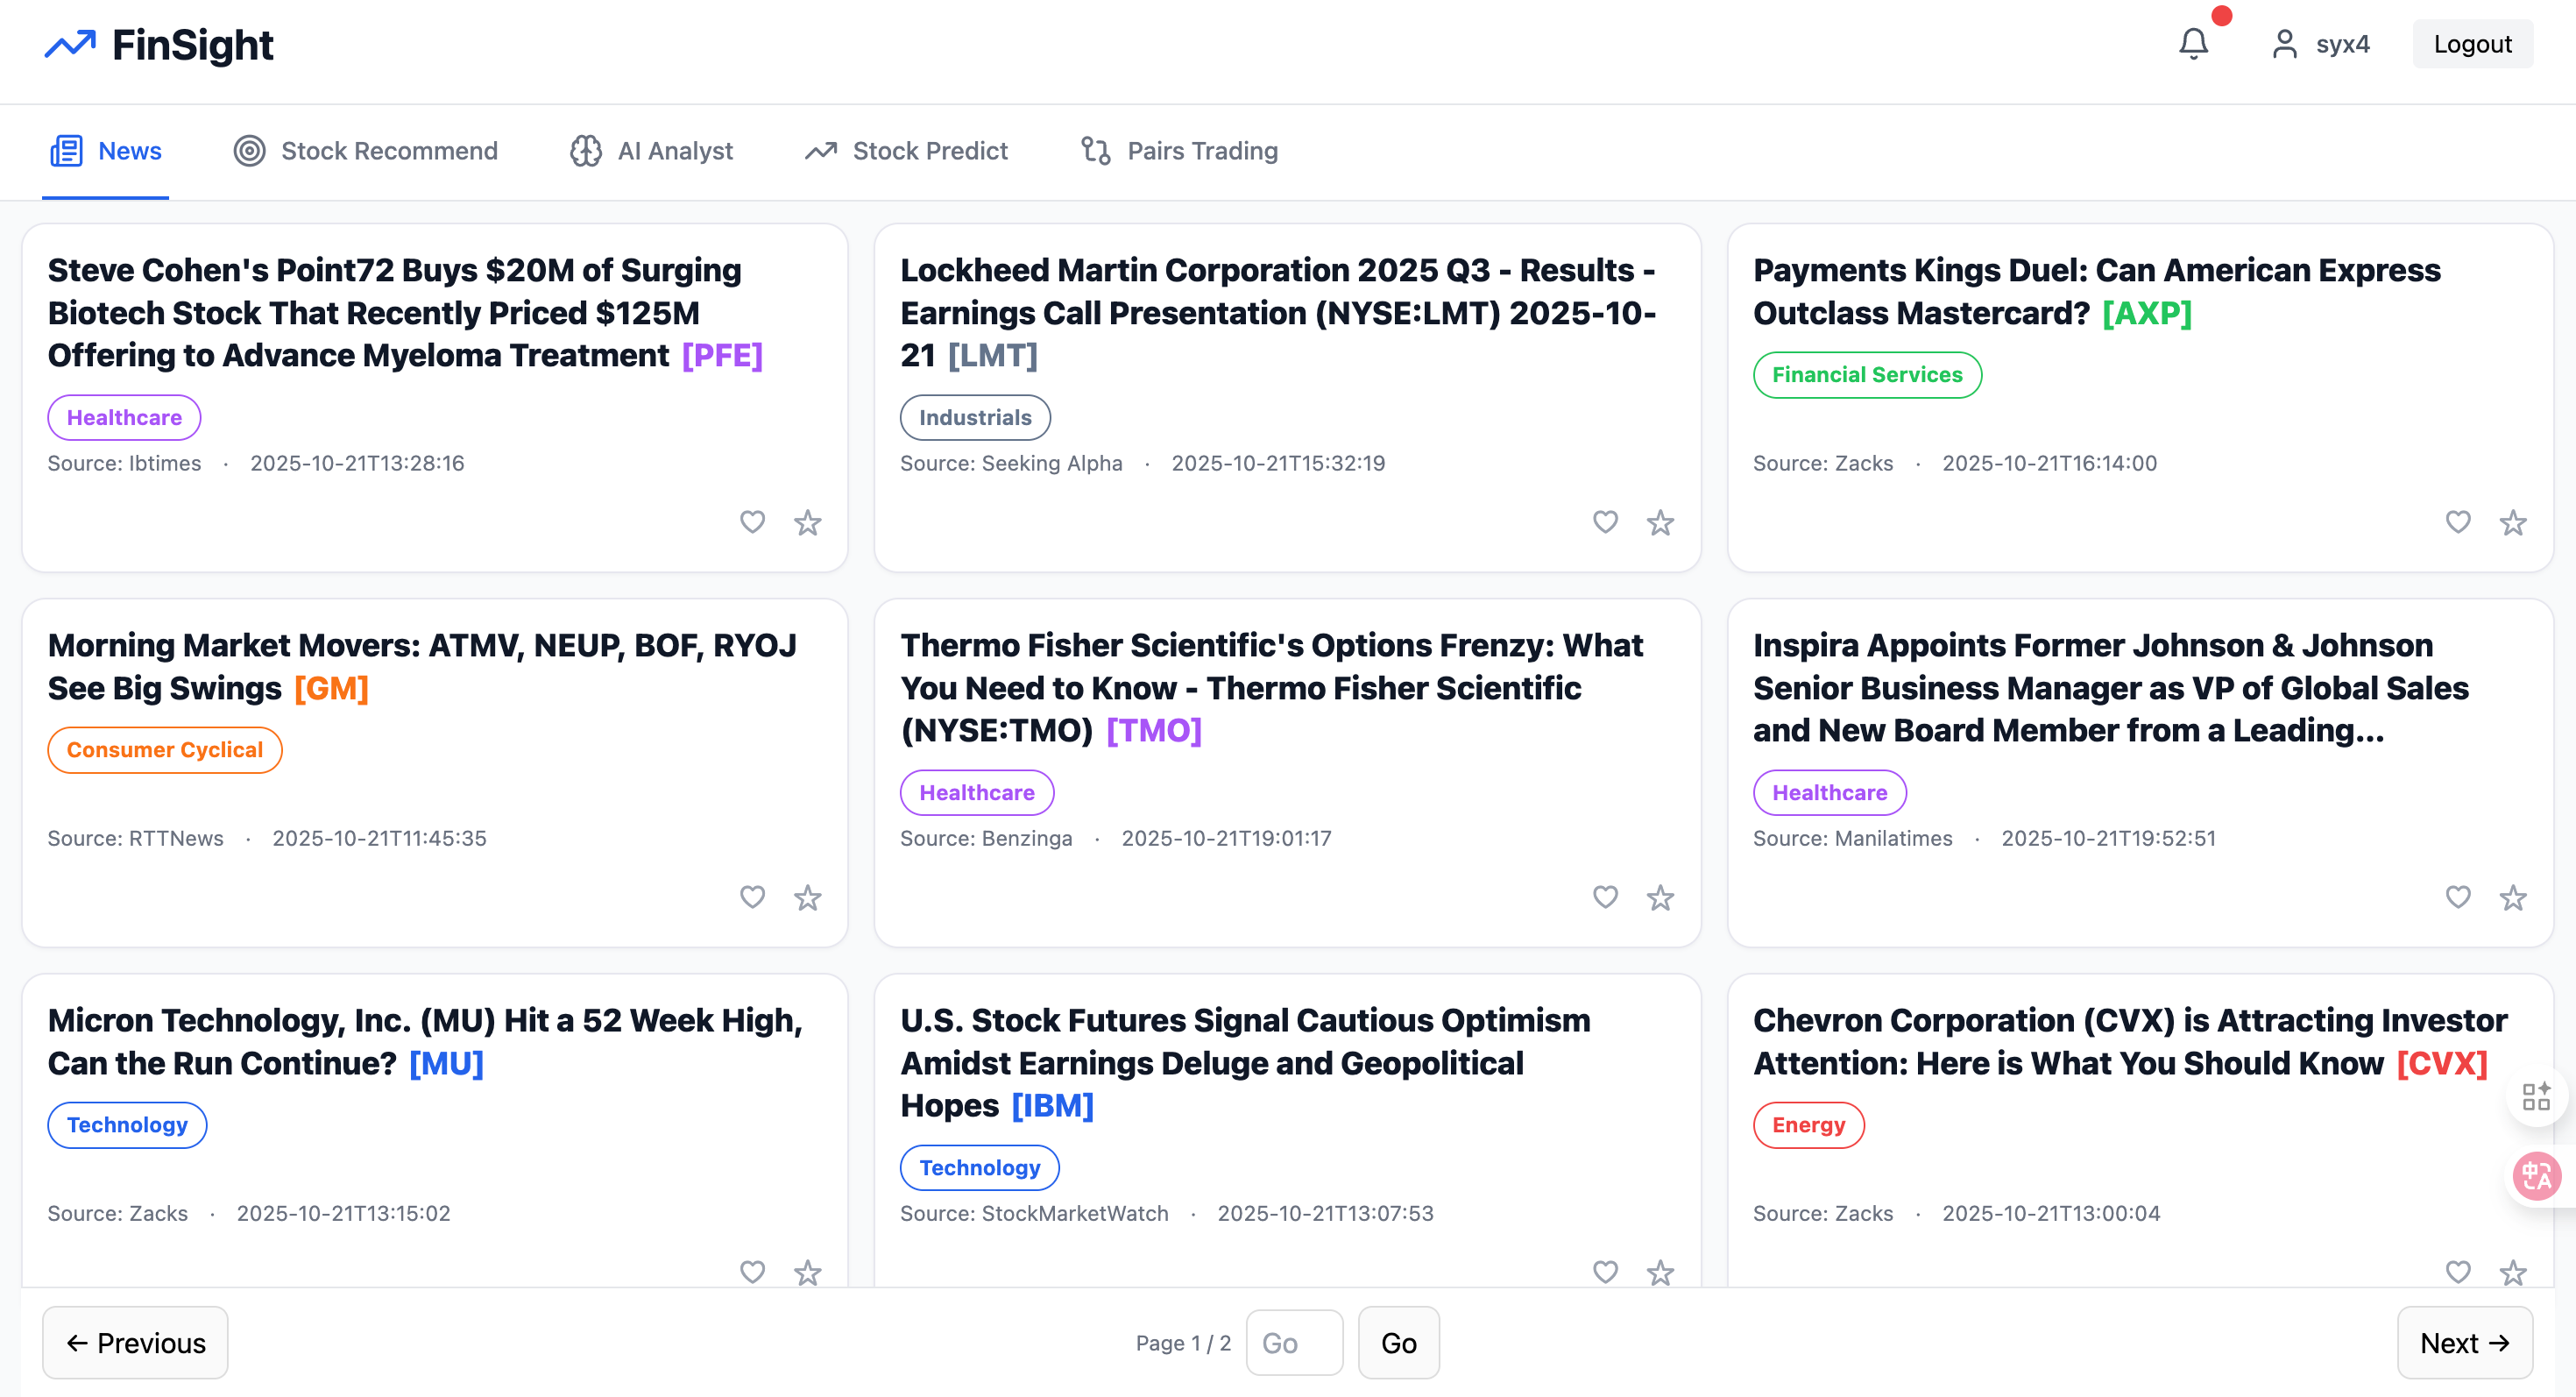
\includegraphics[width=0.9\textwidth]{images/news/page1.png}
% \caption{Initial News Feed Page Showing Personalized News Cards}
% \label{fig:news_page1}
% \end{figure}

% Figure \ref{fig:news_page1} illustrates the main news browsing interface, rendered in a \(3\times3\) card grid layout with smooth pagination. Each card presents the article’s title, ticker, sector tag, source, and publication date. The system retrieves these articles from the MongoDB-based news repository and applies the server-side ranking logic described earlier. Users can move between pages using \texttt{Previous}, \texttt{Next}, and direct page jump buttons, with cached navigation to minimize latency.

% When the user reaches the last page and triggers \texttt{Next}, the system enters the \textbf{trickle refresh mode}, dynamically fetching 1–3 new articles based on active tickers and seamlessly appending them to the local corpus. Figure \ref{fig:news_page2} shows the refreshed interface with new, unseen news items loaded.

% \begin{figure}[h]
% \centering
% 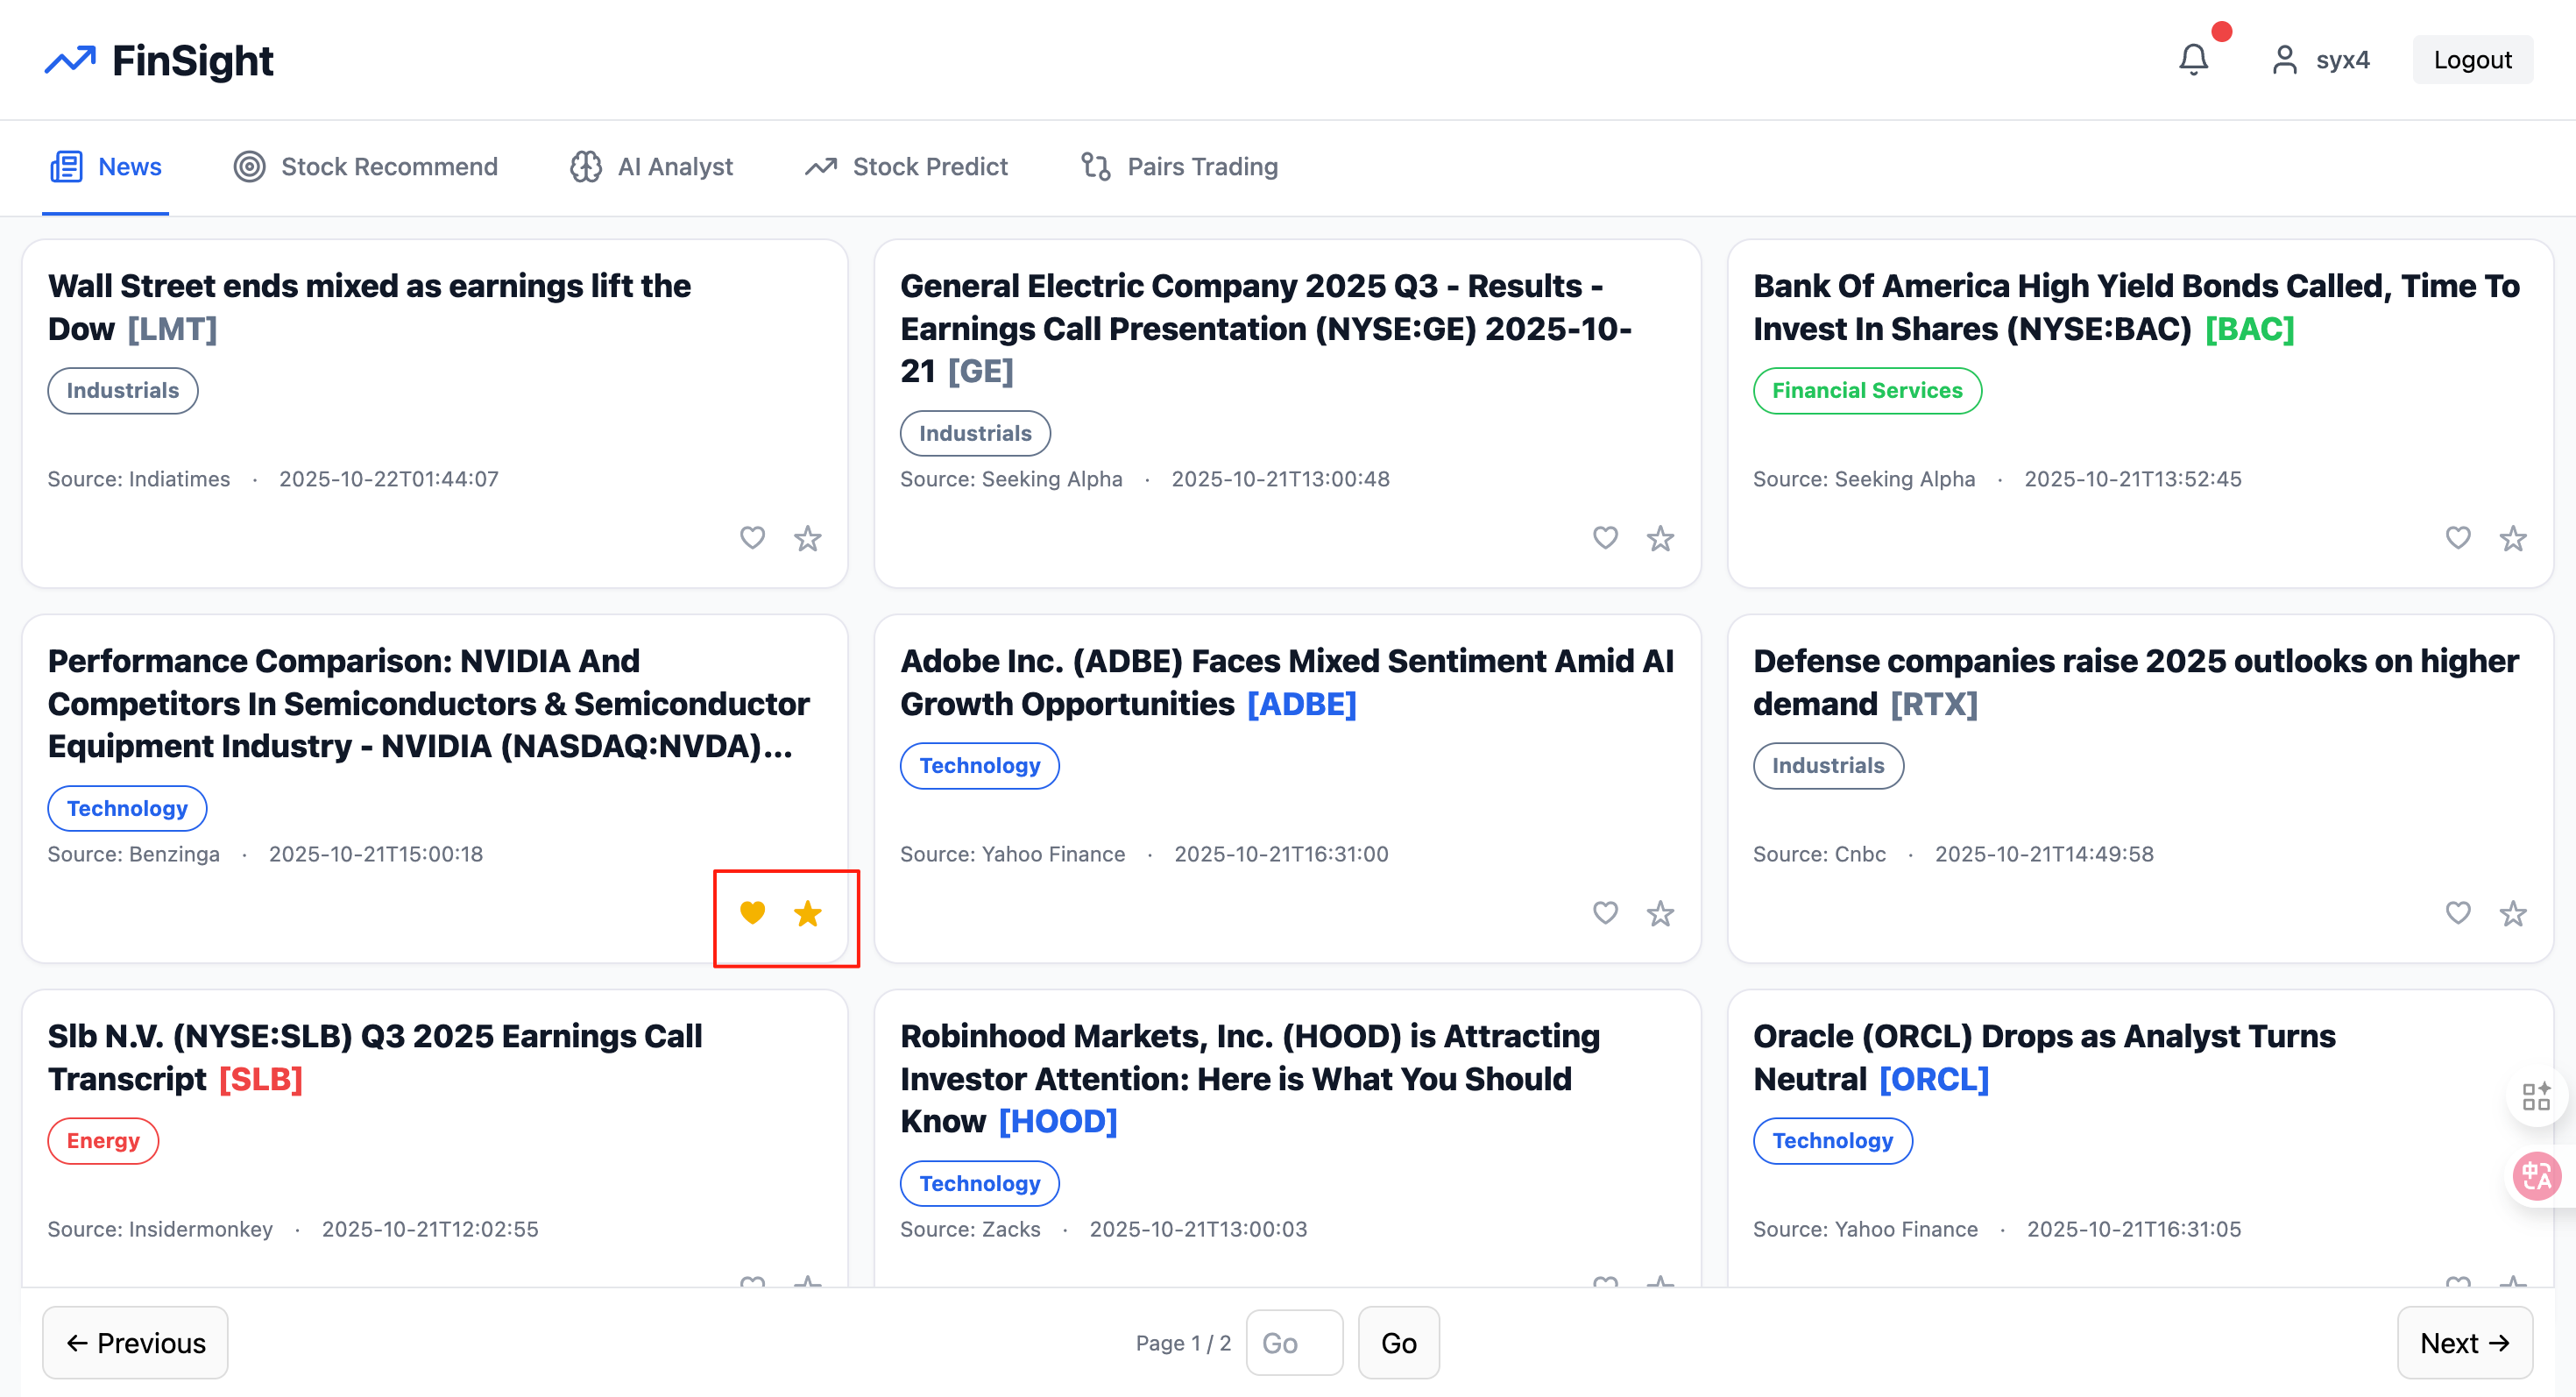
\includegraphics[width=0.9\textwidth]{images/news/page2.png}
% \caption{Trickle Refresh Mode Loading New Articles in Real-Time}
% \label{fig:news_page2}
% \end{figure}

% \textbf{2. User Interaction and Real-Time Vector Updates}

% The front-end enables three types of user interactions: \textbf{click}, \textbf{like}, and \textbf{bookmark}. These actions are recorded in MongoDB (\texttt{EventRepo}) and simultaneously update the user's 64-d semantic and 20-d preference vectors in PostgreSQL. 

% Figures \ref{fig:clk1} and \ref{fig:clk2} depict the process of a user liking a news article. The yellow heart/star icons represent a successful \texttt{like} action, which triggers the backend’s \texttt{update\_prof20\_add()} function in \texttt{PgProfileRepo}, adjusting the relevant preference dimensions.

% \begin{figure}[h]
% \centering
% 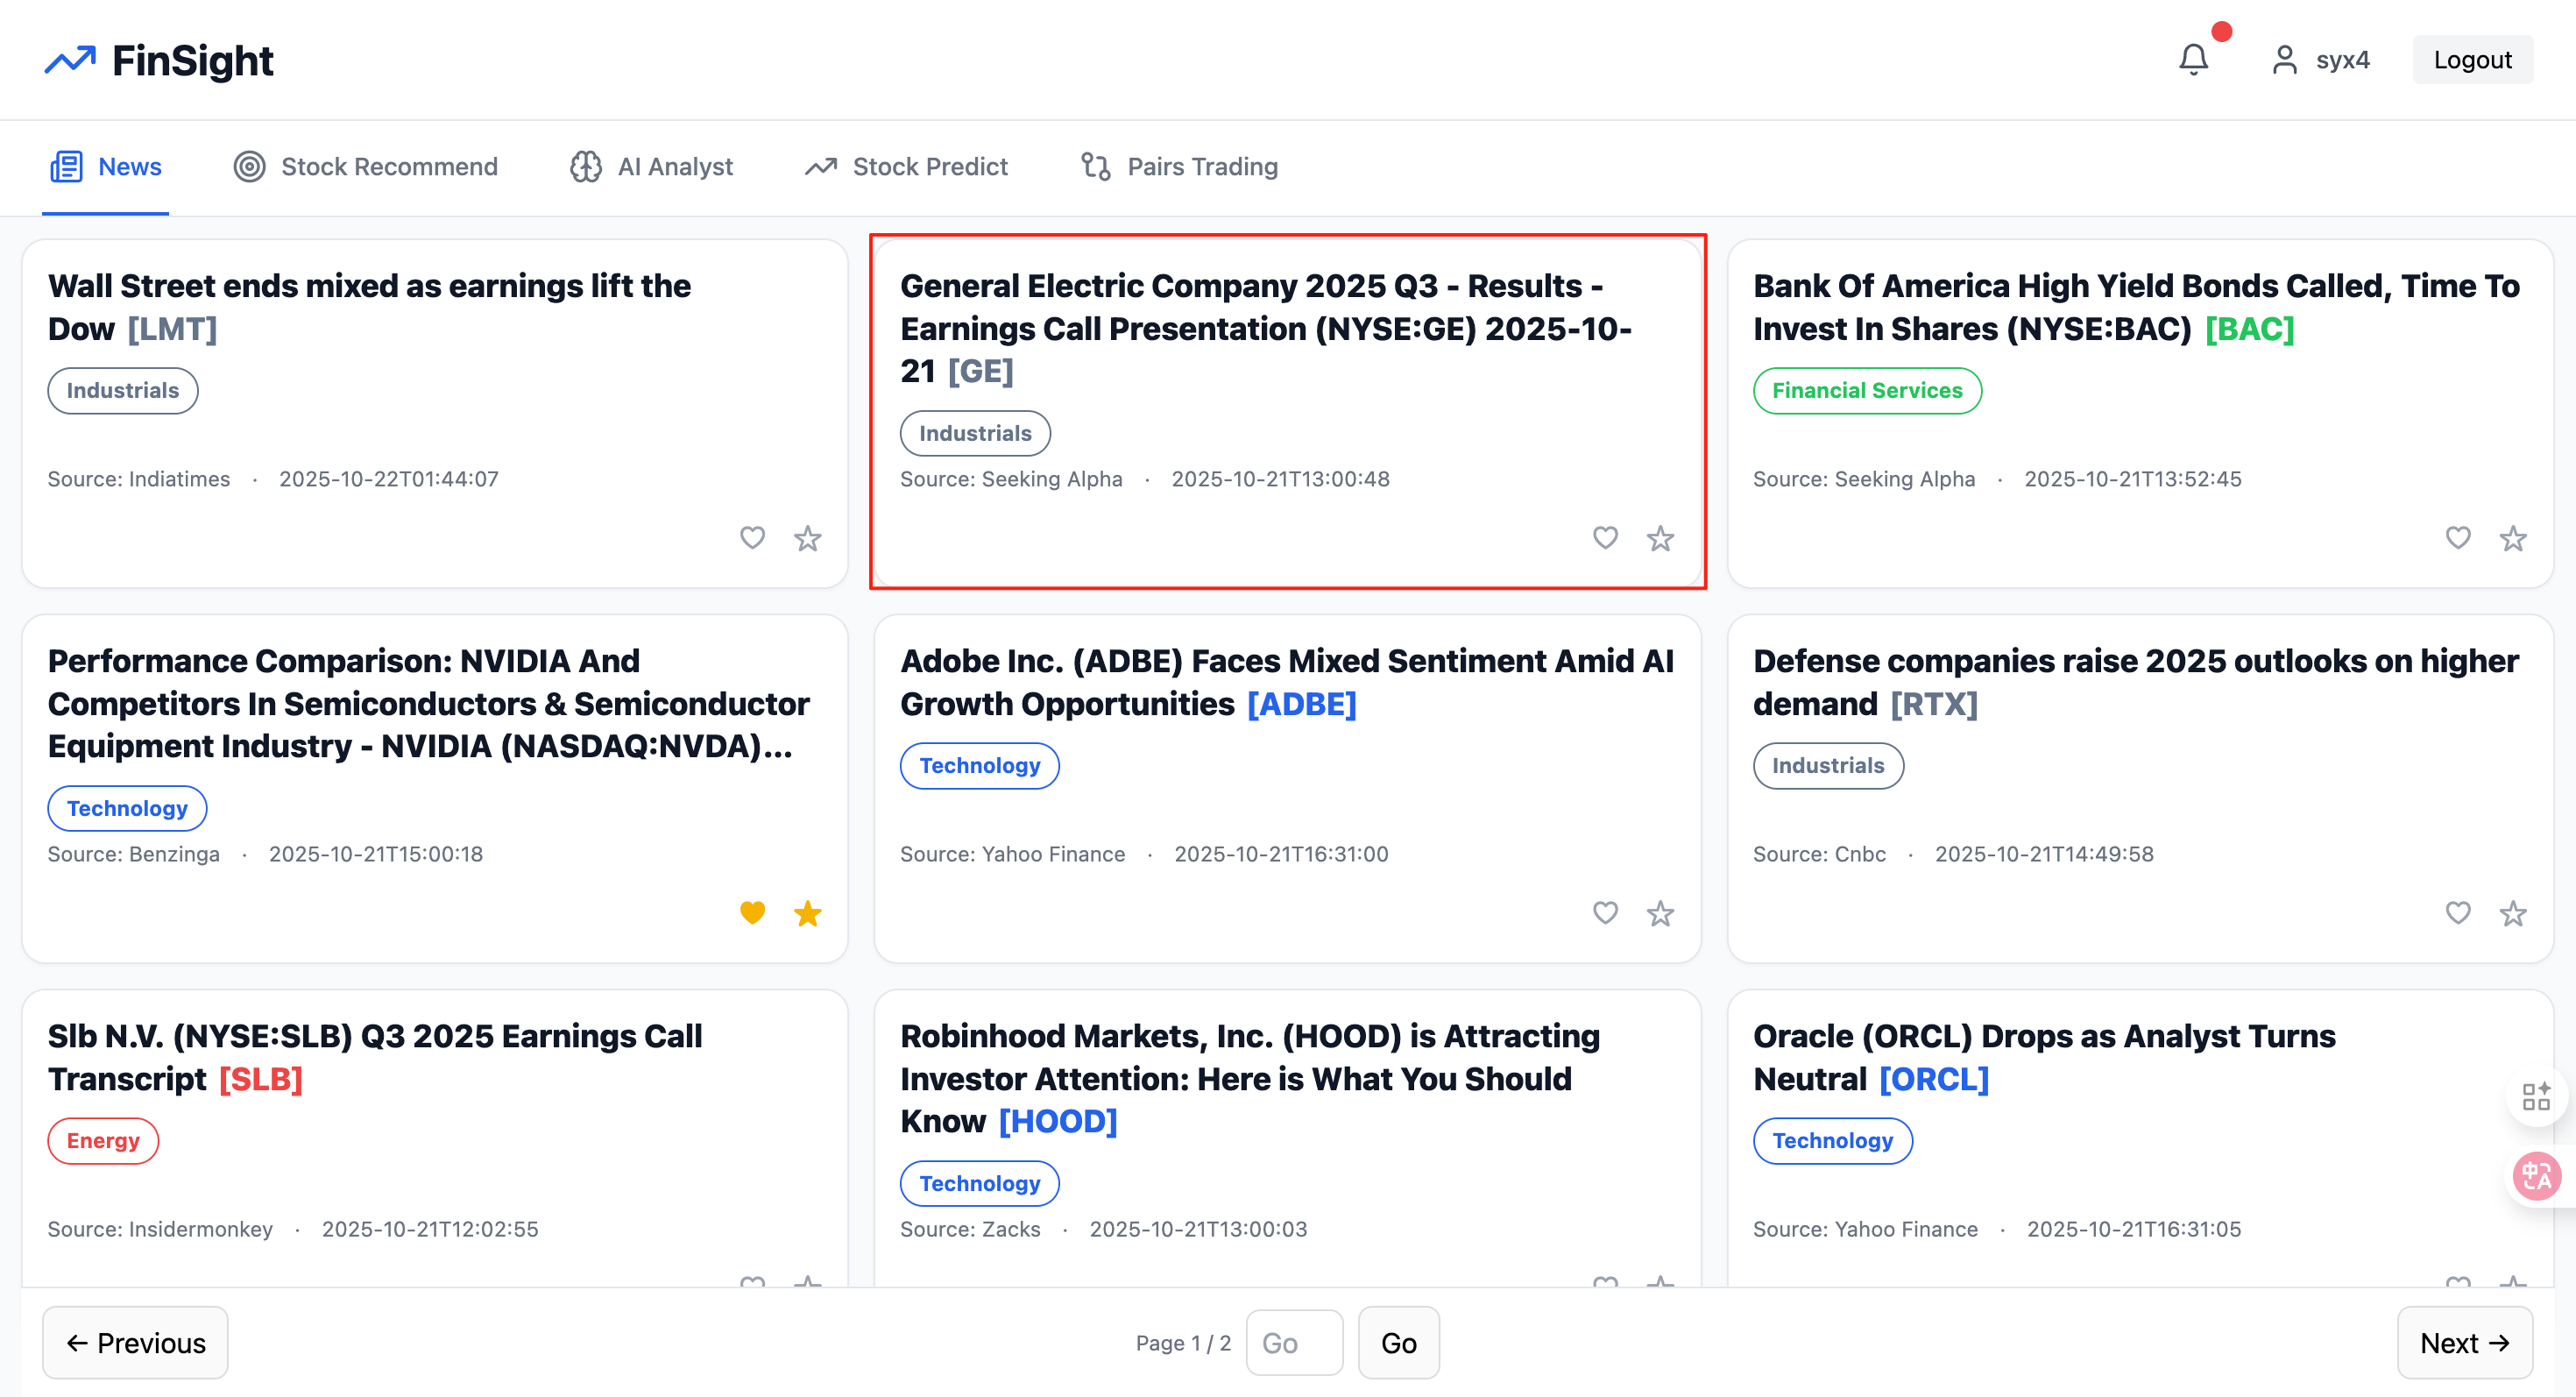
\includegraphics[width=0.8\textwidth]{images/news/clk1.png}
% \caption{User Performing Like and Bookmark Action on News Item}
% \label{fig:clk1}
% \end{figure}

% \begin{figure}[h]
% \centering
% 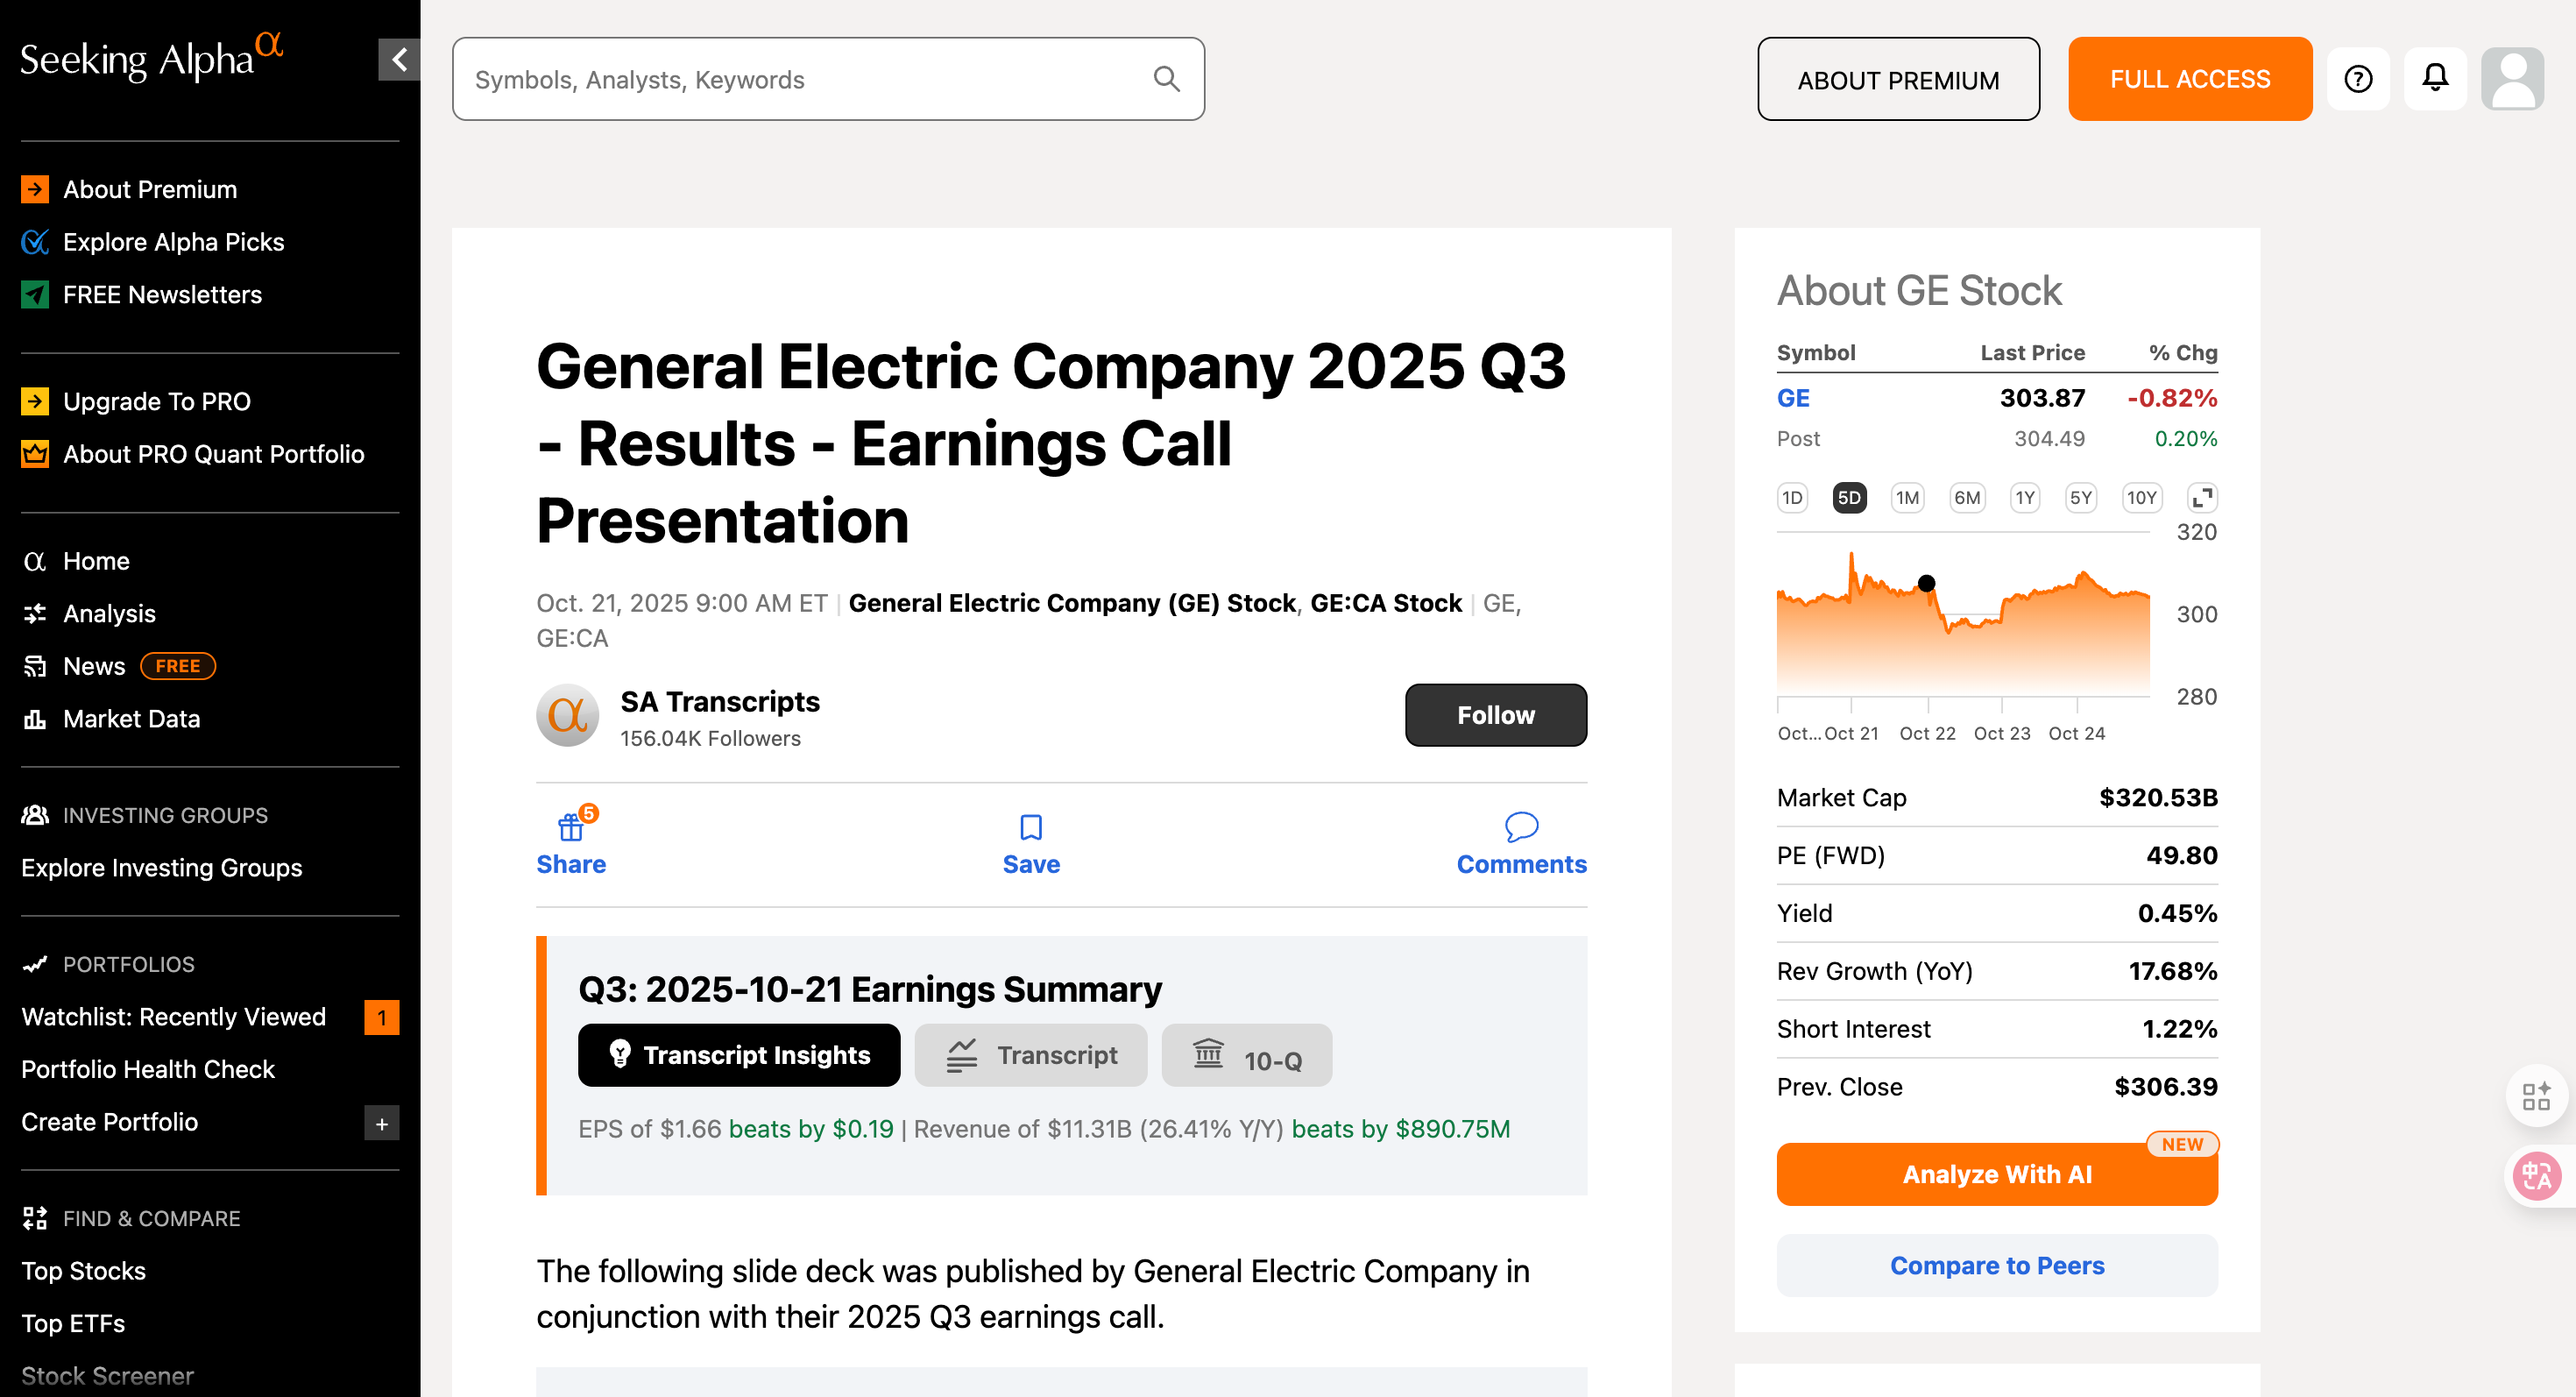
\includegraphics[width=0.8\textwidth]{images/news/clk2.png}
% \caption{Updated Preference Reflected in UI and Database}
% \label{fig:clk2}
% \end{figure}

% \textbf{3. Back-End Profile Evolution Verification}

% To verify personalization, we track vector changes before and after user actions. Figures \ref{fig:20d1} and \ref{fig:20d2} show the evolution of the 20-dimensional preference vector (\texttt{profile\_vector\_20d}), where the highlighted component (e.g., industrial sector dimension) increased after the user liked a relevant article.

% \begin{figure}[h]
% \centering
% 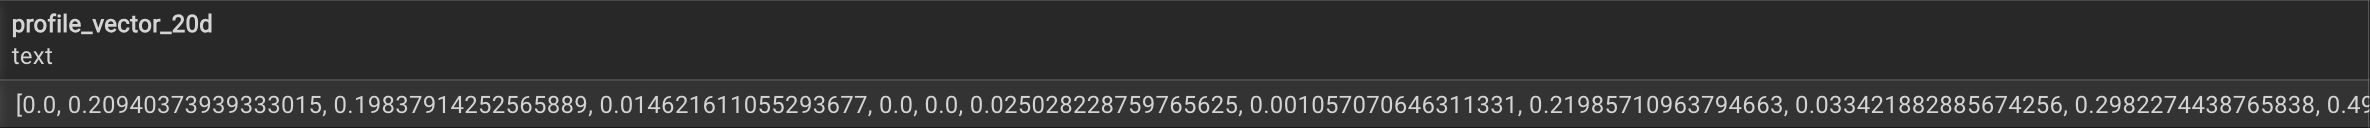
\includegraphics[width=0.8\textwidth]{images/news/20d1.png}
% \caption{User 20-D Preference Vector Before Interaction}
% \label{fig:20d1}
% \end{figure}

% \begin{figure}[h]
% \centering
% 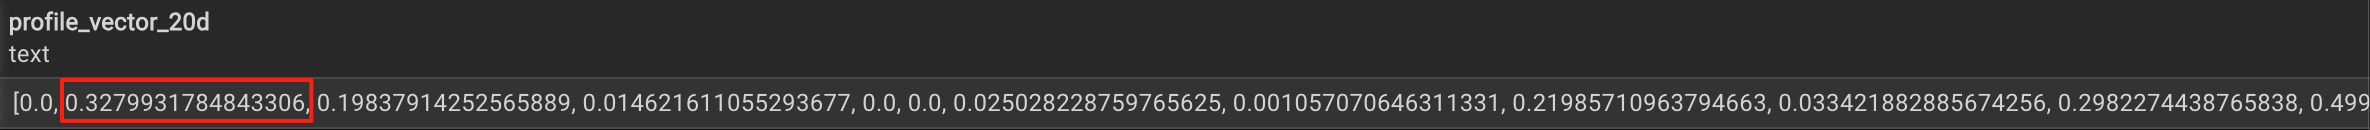
\includegraphics[width=0.8\textwidth]{images/news/20d2.png}
% \caption{User 20-D Preference Vector After Interaction: Technology Weight Increased}
% \label{fig:20d2}
% \end{figure}

% Similarly, Figures \ref{fig:64d1} and \ref{fig:64d2} present the 64-dimensional short-term semantic embedding (\texttt{user\_semantic\_64d\_short}), which undergoes slight EMA-based shifts reflecting the article’s content vector. These changes collectively guide ranking adjustments for subsequent recommendations.

% \textbf{4. Live Personalization and Feedback Loop}

% As the vectors evolve, the ranking service recalculates cosine similarities between the updated user vector \(\mathbf{u}\) and article vectors \(\mathbf{p}_a\), reordering results on subsequent refreshes. This ensures that after a user interacts with specific sectors (e.g., Technology or Industrials), the following pages emphasize those preferences while maintaining diversity.

% \begin{figure}[h]
% \centering
% 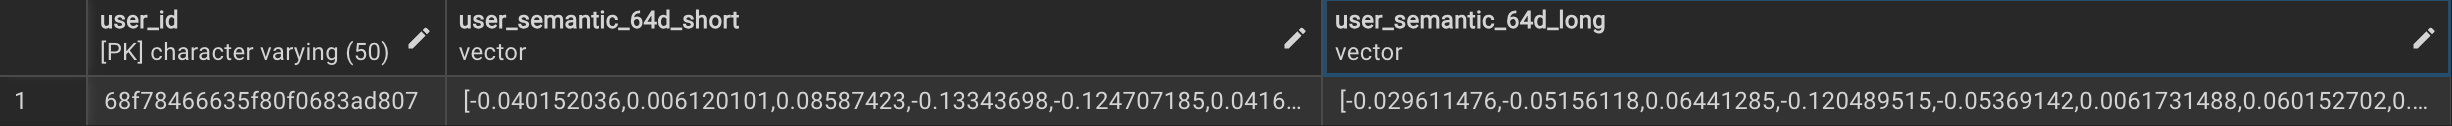
\includegraphics[width=0.8\textwidth]{images/news/64d1.png}
% \caption{User 64-D Semantic Vector Before Interaction}
% \label{fig:64d1}
% \end{figure}

% \begin{figure}[h]
% \centering
% 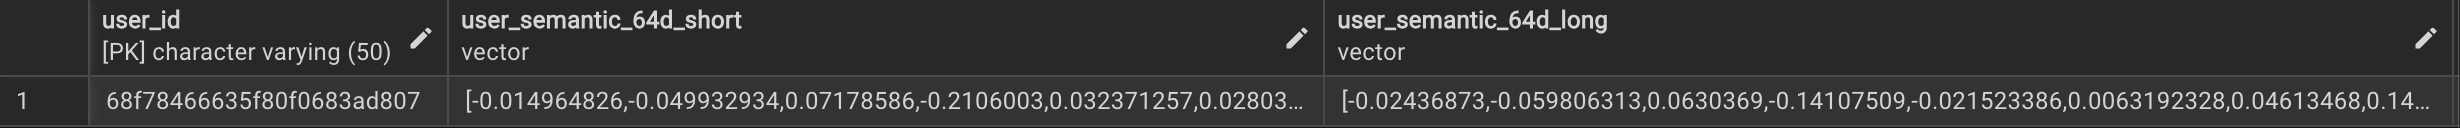
\includegraphics[width=0.8\textwidth]{images/news/64d2.png}
% \caption{User 64-D Semantic Vector After Interaction: Content-Driven Update Applied(click)}
% \label{fig:64d2}
% \end{figure}



% \subsection{Technical Validation and Performance}

% \begin{table}[h]
% \centering
% \caption{System Component Integration Validation for News Module}
% \begin{tabular}{|p{5cm}|p{8cm}|}
% \hline
% \textbf{Component} & \textbf{Validation Result} \\
% \hline
% Frontend-Backend Integration & React front-end communicates with FastAPI backend seamlessly; event logging and vector updates confirmed in real time. \\
% \hline
% Data Pipeline Integration & Google RSS and Marketaux APIs successfully fetch fresh news data; MongoDB upsert and de-duplication verified. \\
% \hline
% Database Schema Consistency & PostgreSQL 64d/20d vectors and JSON mirrors remain synchronized; type safety verified after feedback actions. \\
% \hline
% Exclude-Seen and Ranking & Sliding-window filtering correctly removes recently read articles; ranking reflects both recency and preference match. \\
% \hline
% System Latency & Typical \texttt{/rec/user/news} response time: 120–180 ms (cached mode); under 250 ms with refresh-enabled fetch. \\
% \hline
% \end{tabular}
% \end{table}

% \textbf{User Experience and Responsiveness}

% The interface achieves high responsiveness and transparency:
% \begin{itemize}
% \item Instant page transitions with cached data and async re-ranking
% \item Dynamic icon toggling for likes/bookmarks without reloads
% \item Smooth integration of new articles under \texttt{refresh=1}
% \item Real-time user preference shaping reflected in subsequent recommendations
% \end{itemize}



\section{News Browsing Module}

\subsection{System Functionality Demonstration}

The News Browsing Module has been fully implemented and integrated into the FinSight platform. This section demonstrates the key functionalities of the module—news fetching, ranking, user interaction, and personalization—alongside actual screenshots from the deployed system.

\textbf{1. Core Interface and Pagination System}

\begin{figure}[H]
  \centering
  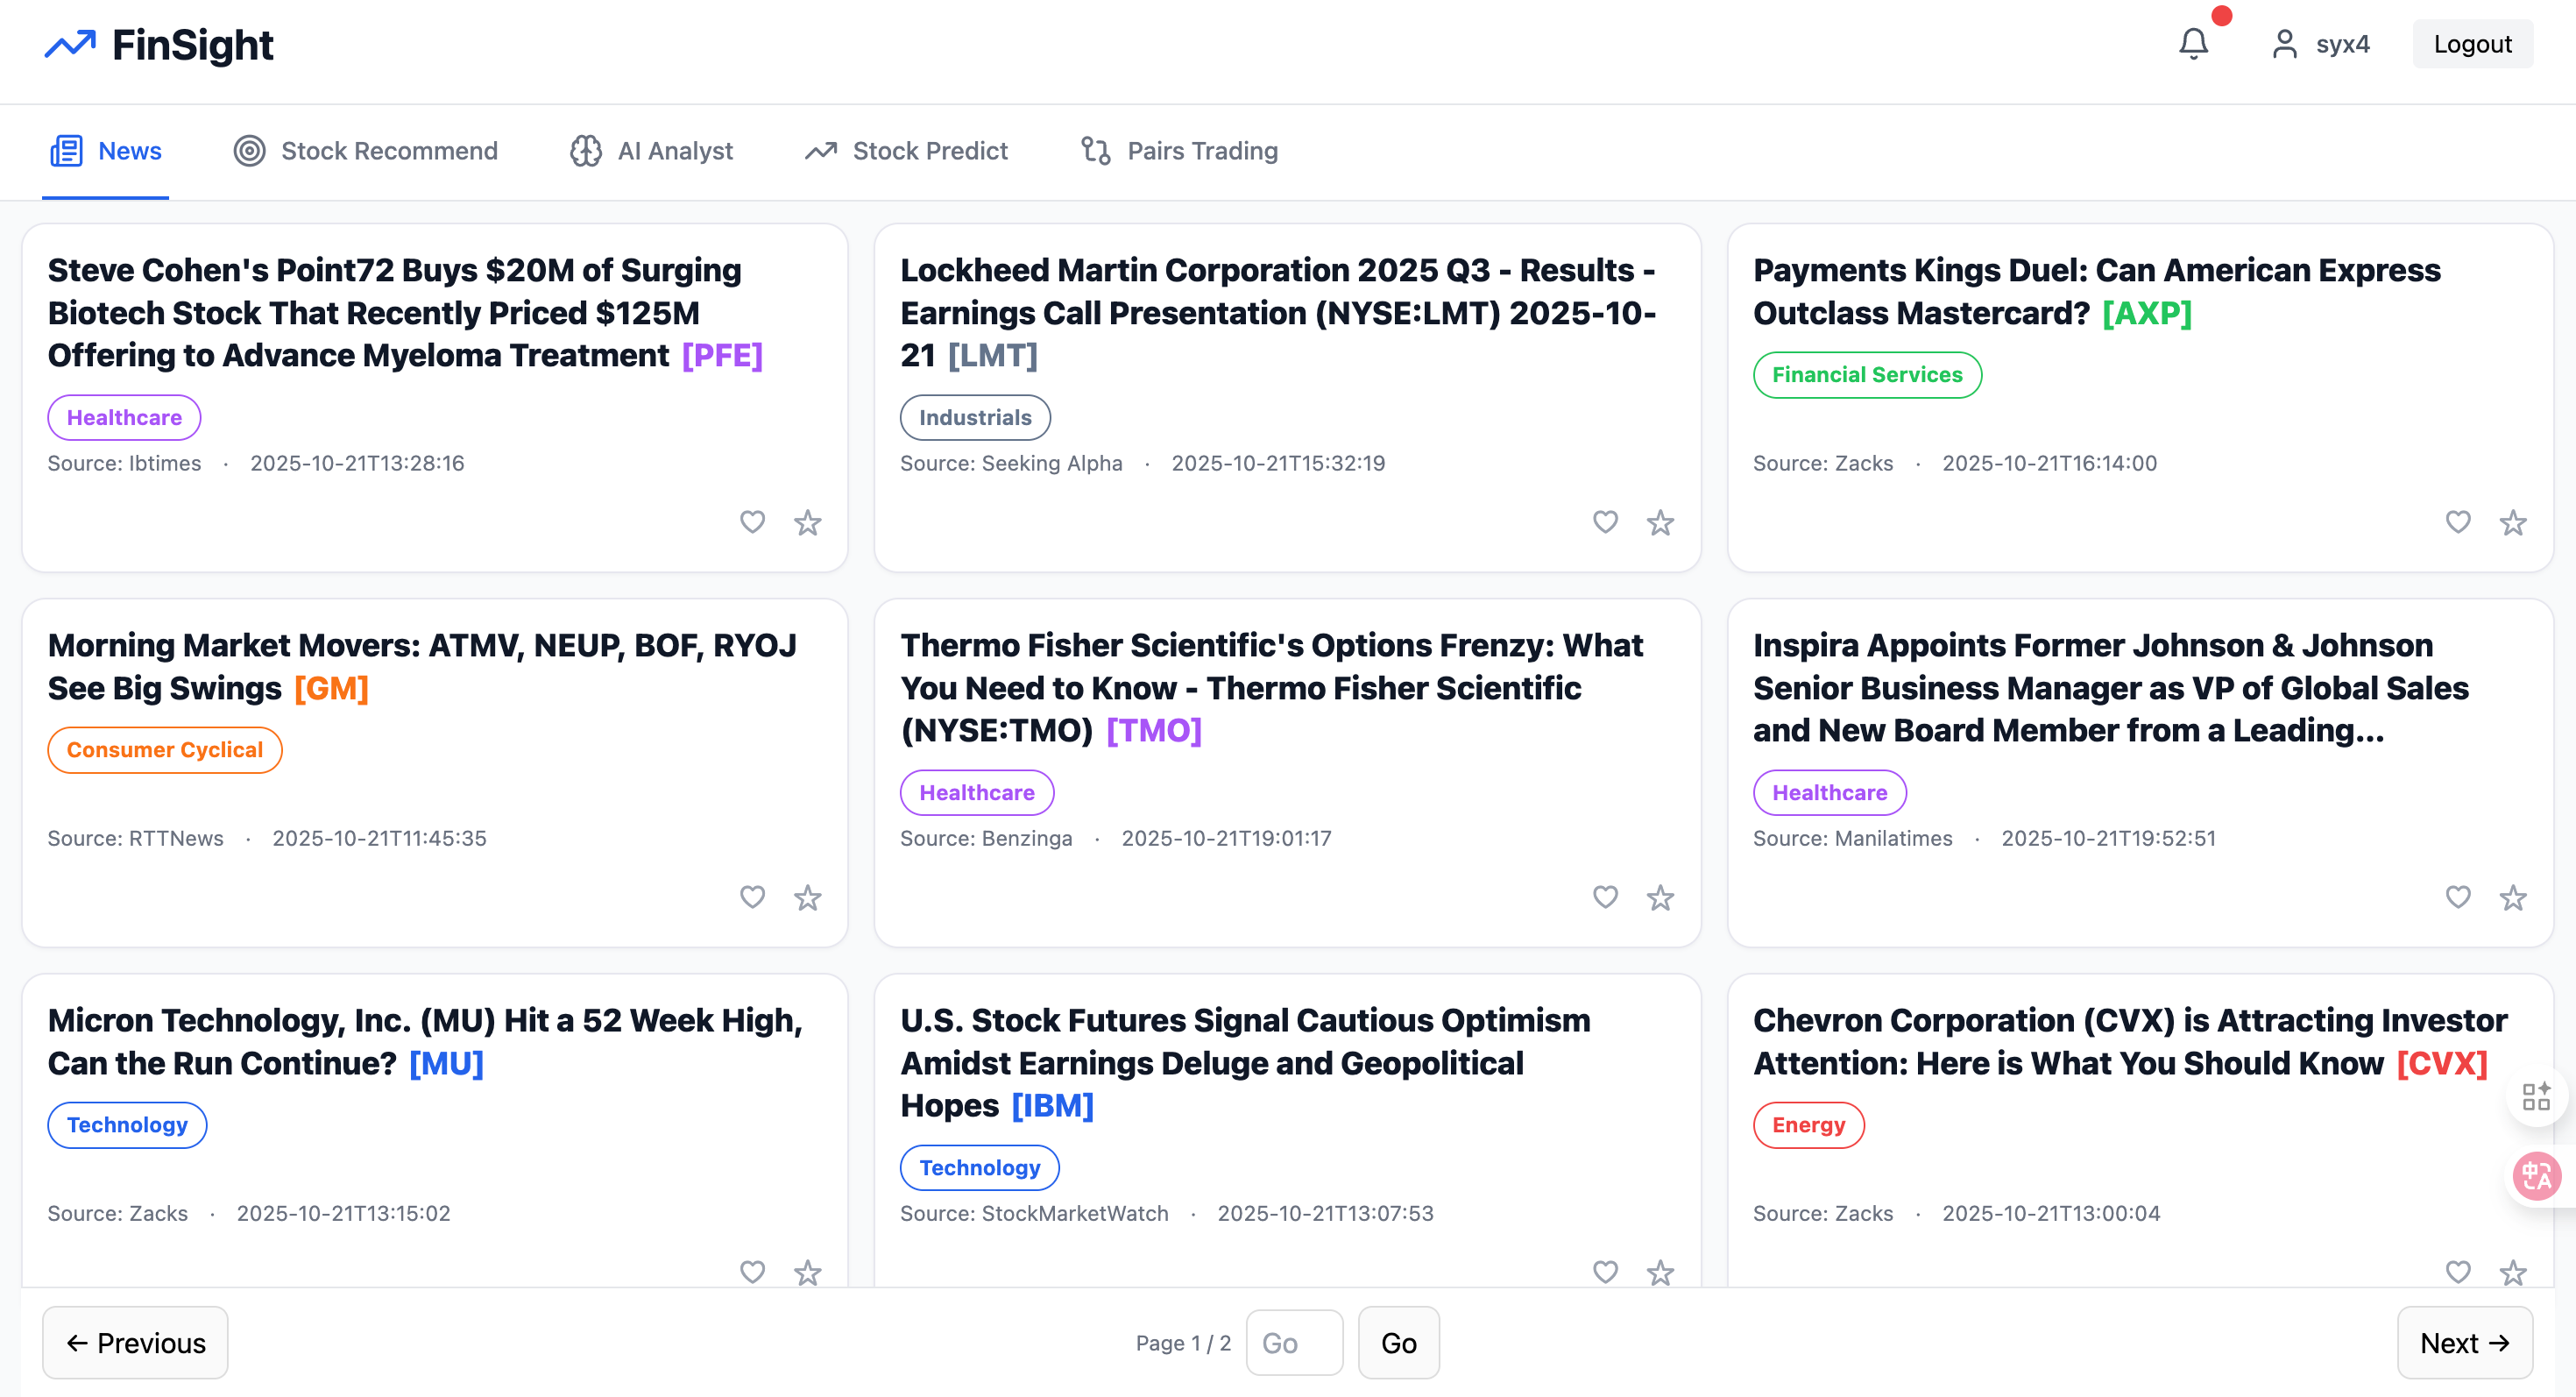
\includegraphics[width=0.92\textwidth]{images/news/page1.png}
  \caption{Initial News Feed Page Showing Personalized News Cards}
  \label{fig:news_page1}
\end{figure}

Figure~\ref{fig:news_page1} illustrates the main news browsing interface, rendered in a \(3\times3\) card grid layout with smooth pagination. Each card presents the article’s title, ticker, sector tag, source, and publication date. The system retrieves these articles from the MongoDB-based news repository and applies the server-side ranking logic described earlier. Users can move between pages using \texttt{Previous}, \texttt{Next}, and direct page jump buttons, with cached navigation to minimize latency.

When the user reaches the last page and triggers \texttt{Next}, the system enters the \textbf{trickle refresh mode}, dynamically fetching 1–3 new articles based on active tickers and seamlessly appending them to the local corpus.

\begin{figure}[H]
  \centering
  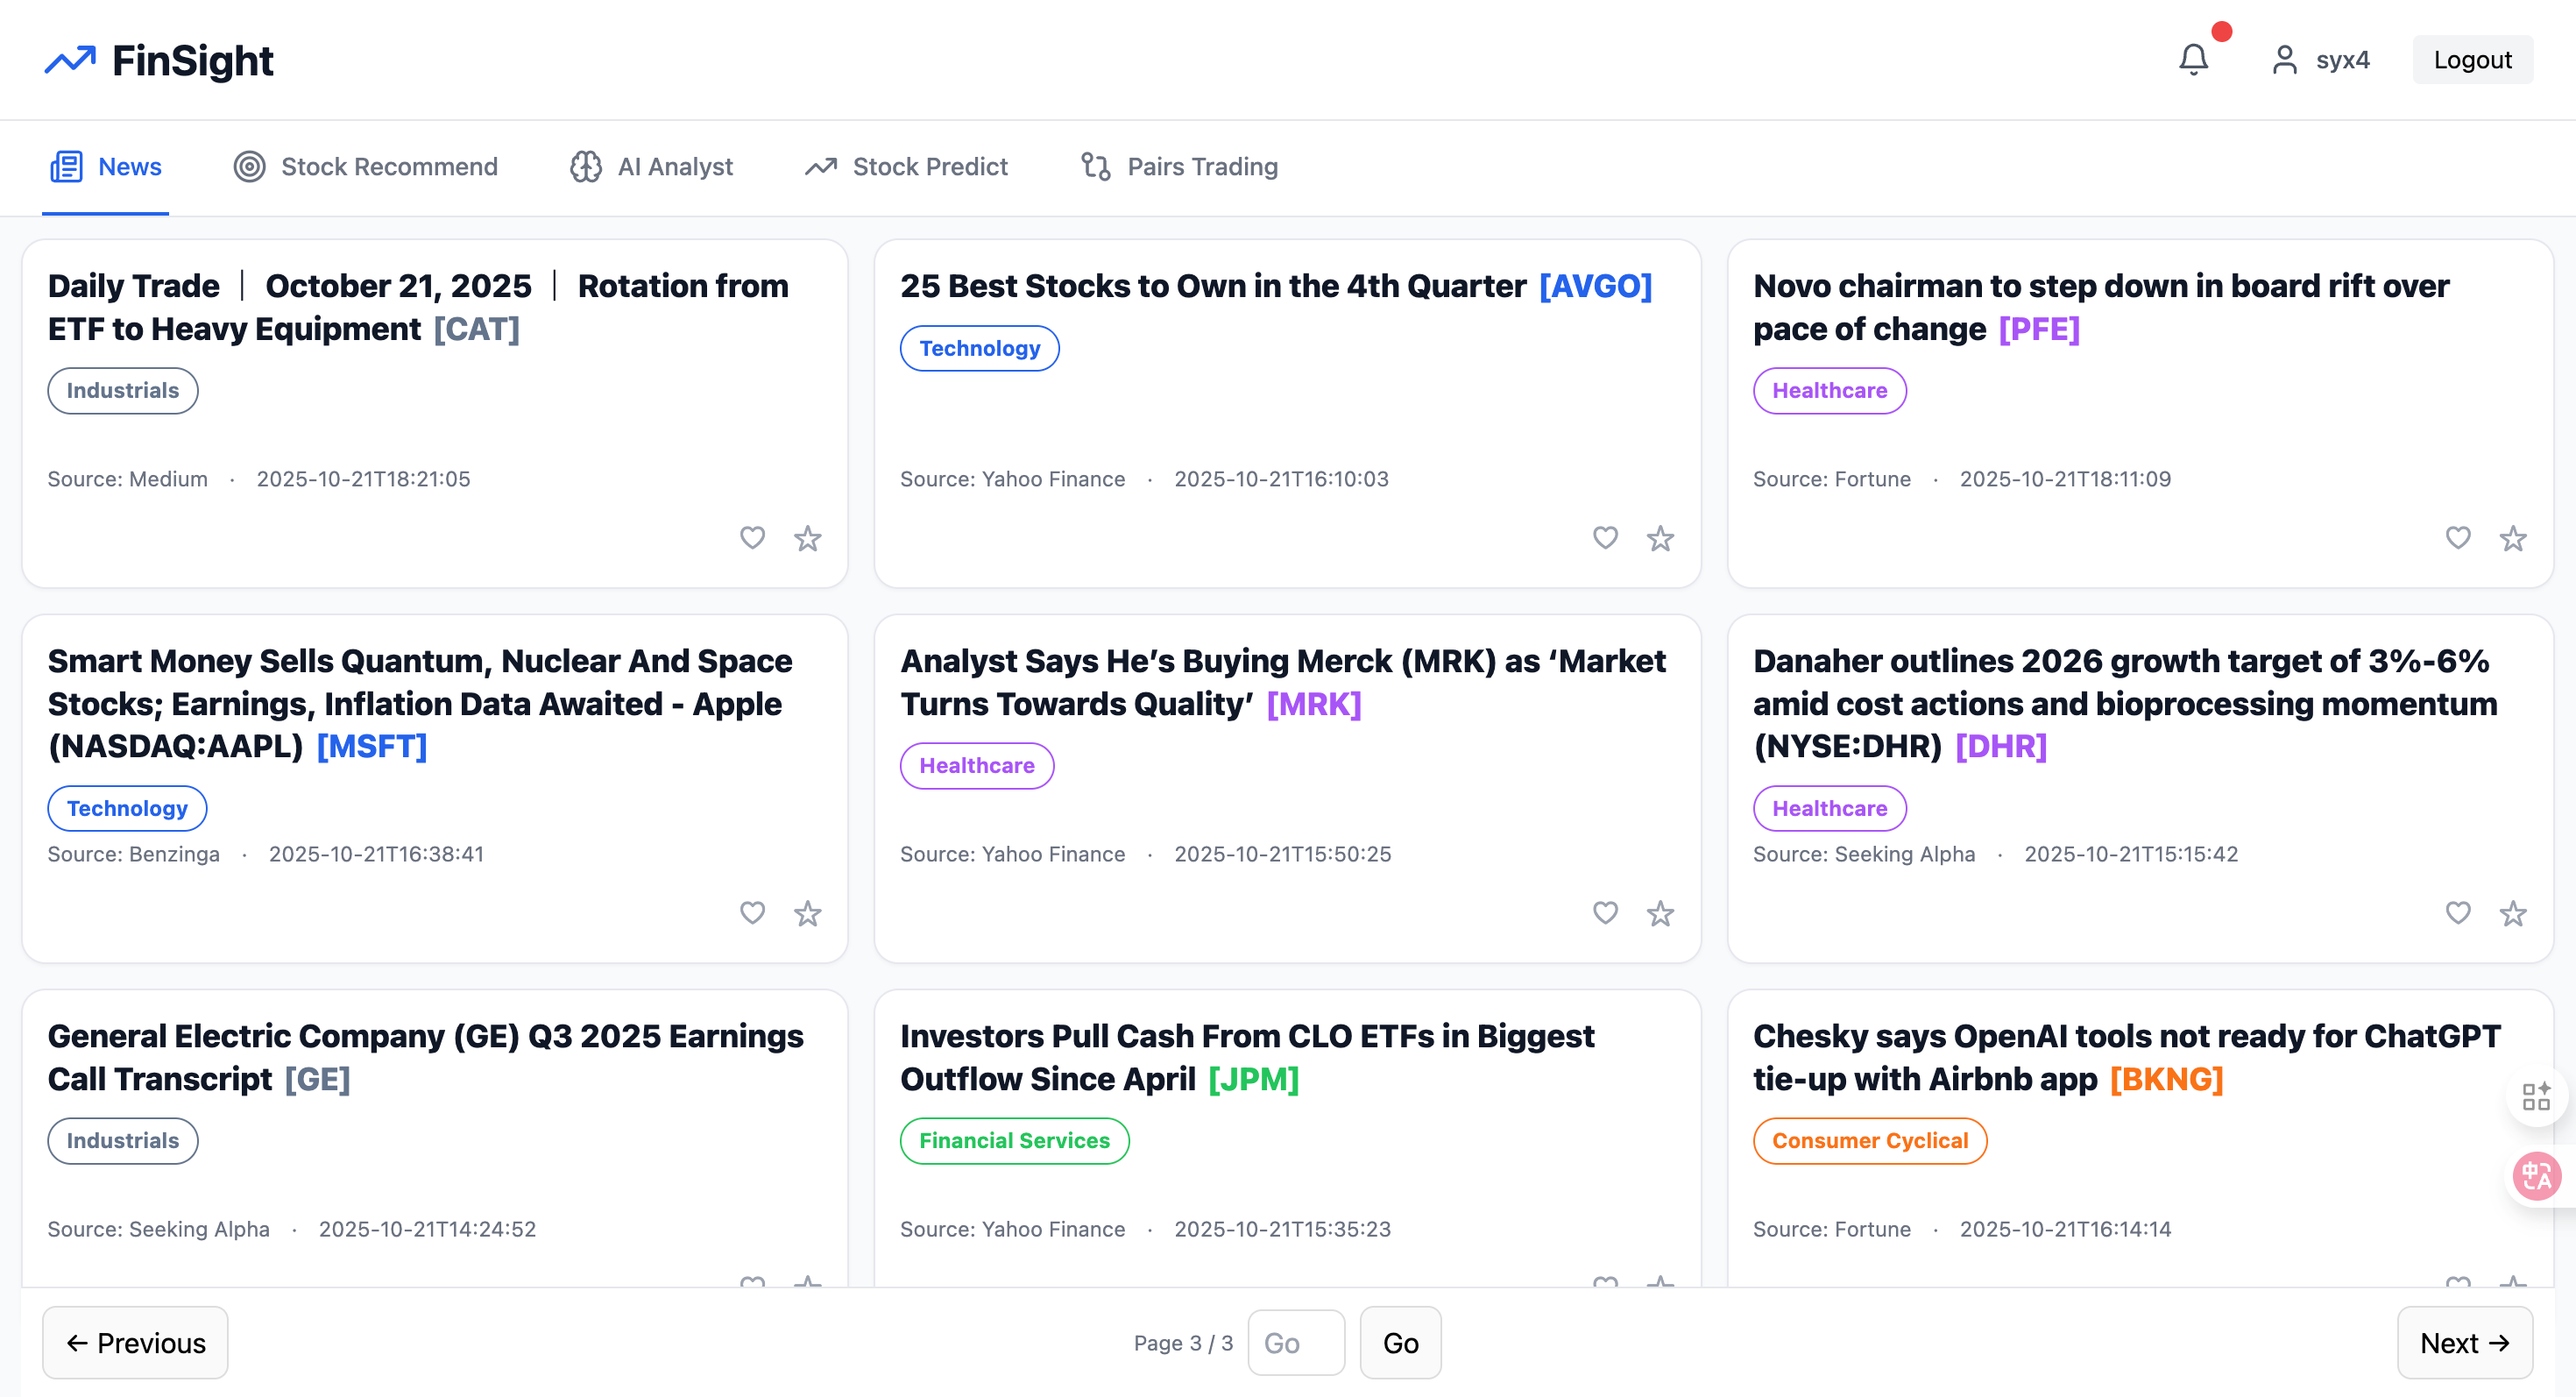
\includegraphics[width=0.92\textwidth]{images/news/refresh.png}
  \caption{Trickle Refresh Mode Loading New Articles in Real-Time}
  \label{fig:refresh}
\end{figure}

\textbf{2. User Interaction and Real-Time Vector Updates}

The front-end enables three types of user interactions: \textbf{click}, \textbf{like}, and \textbf{bookmark}. These actions are recorded in MongoDB (\texttt{EventRepo}) and simultaneously update the user's 64-d semantic and 20-d preference vectors in PostgreSQL.

\begin{figure}[H]
  \centering
  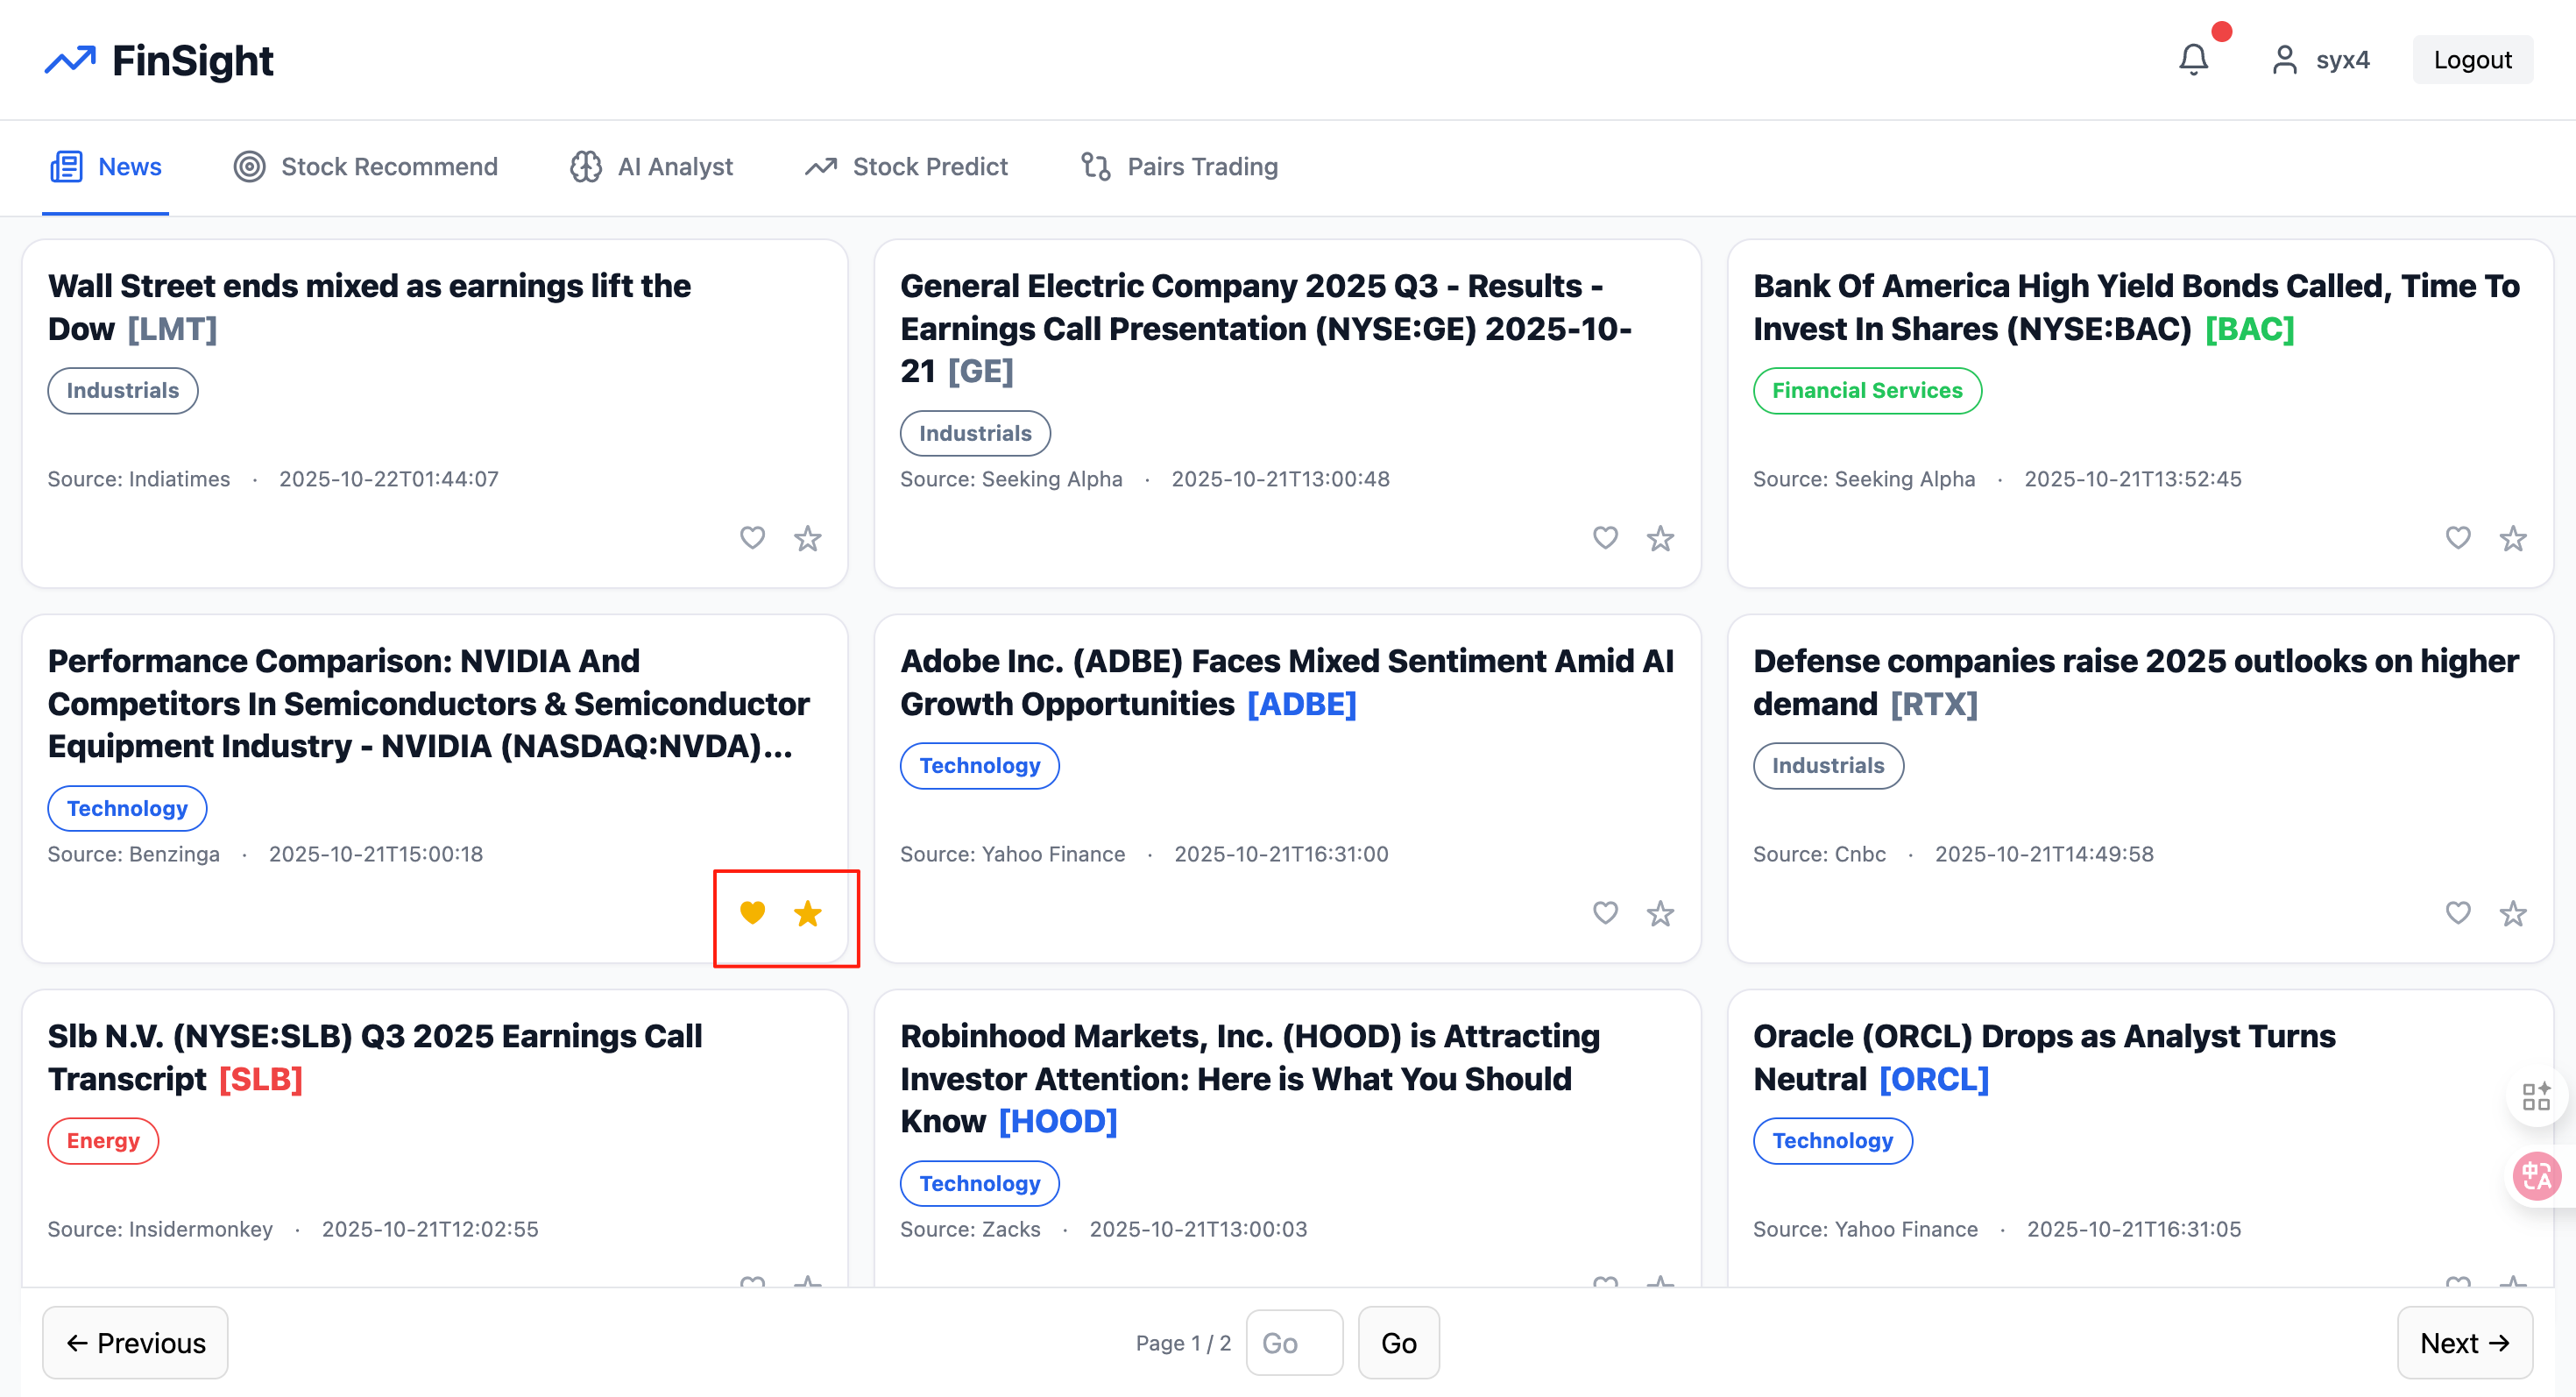
\includegraphics[width=0.82\textwidth]{images/news/page2.png}
  \caption{User Performing Like and Bookmark Action on News Item}
  \label{fig:page2}
\end{figure}


\begin{figure}[H]
  \centering
  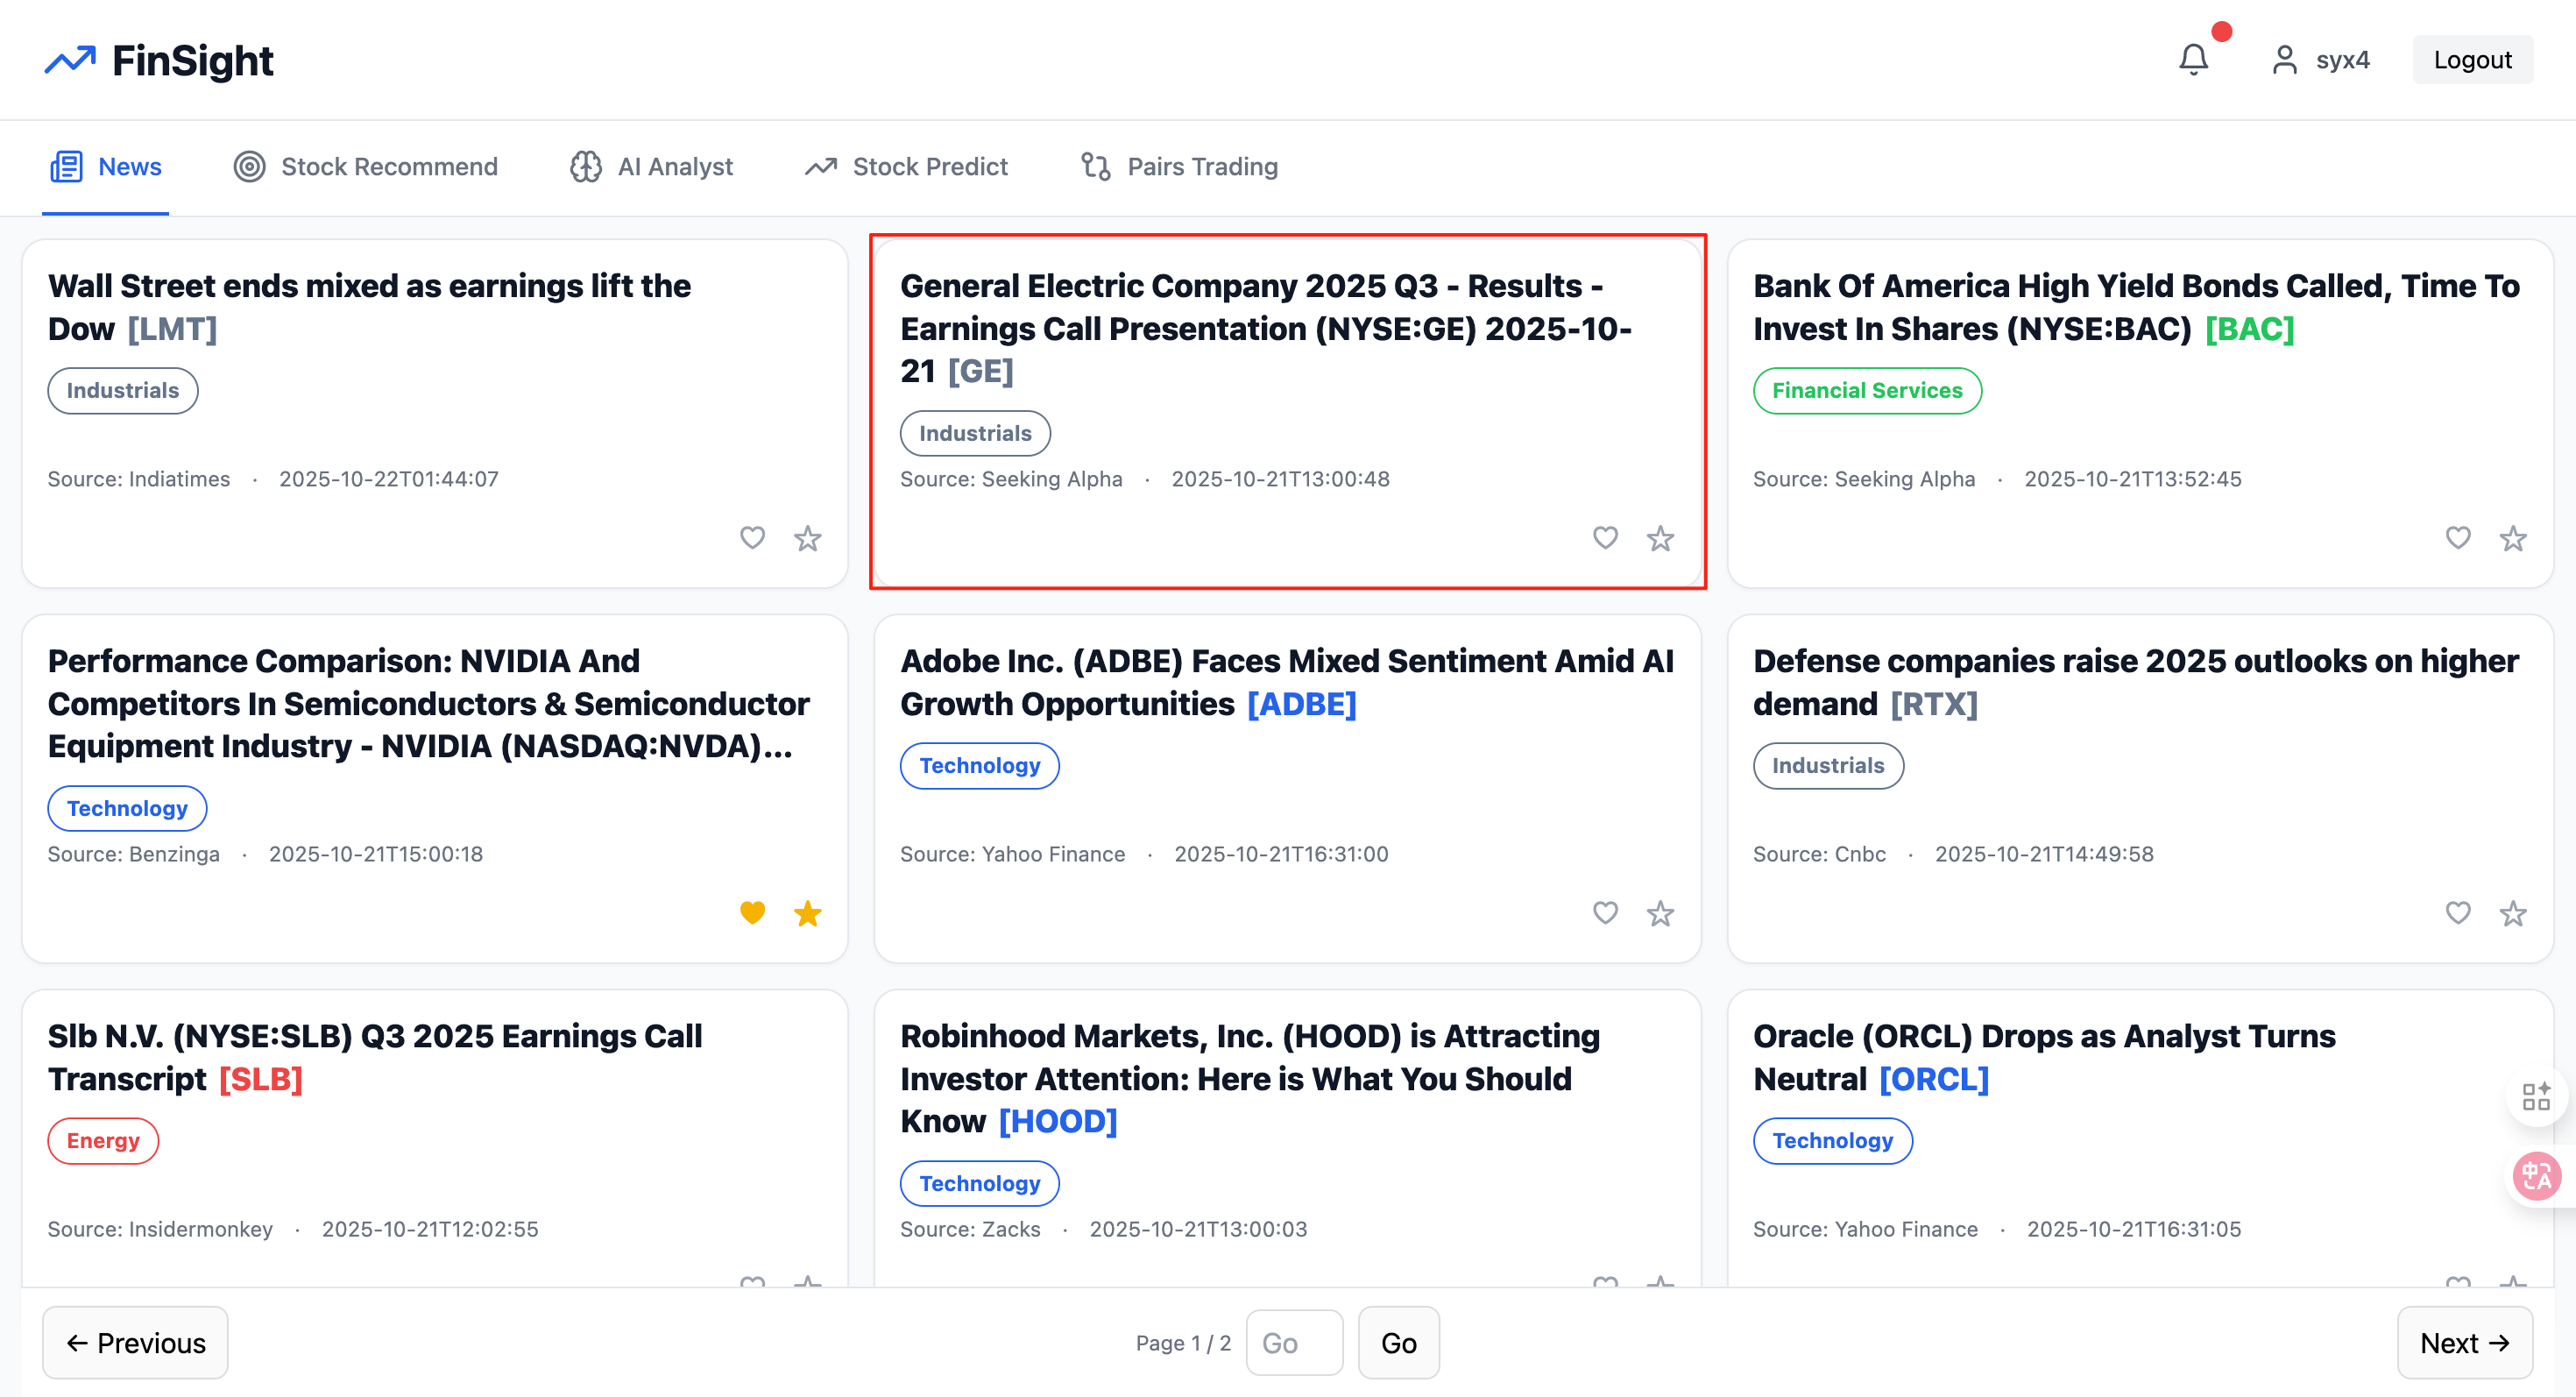
\includegraphics[width=0.82\textwidth]{images/news/clk1.png}
  \caption{Click on news grid}
  \label{fig:clk1}
\end{figure}

\begin{figure}[H]
  \centering
  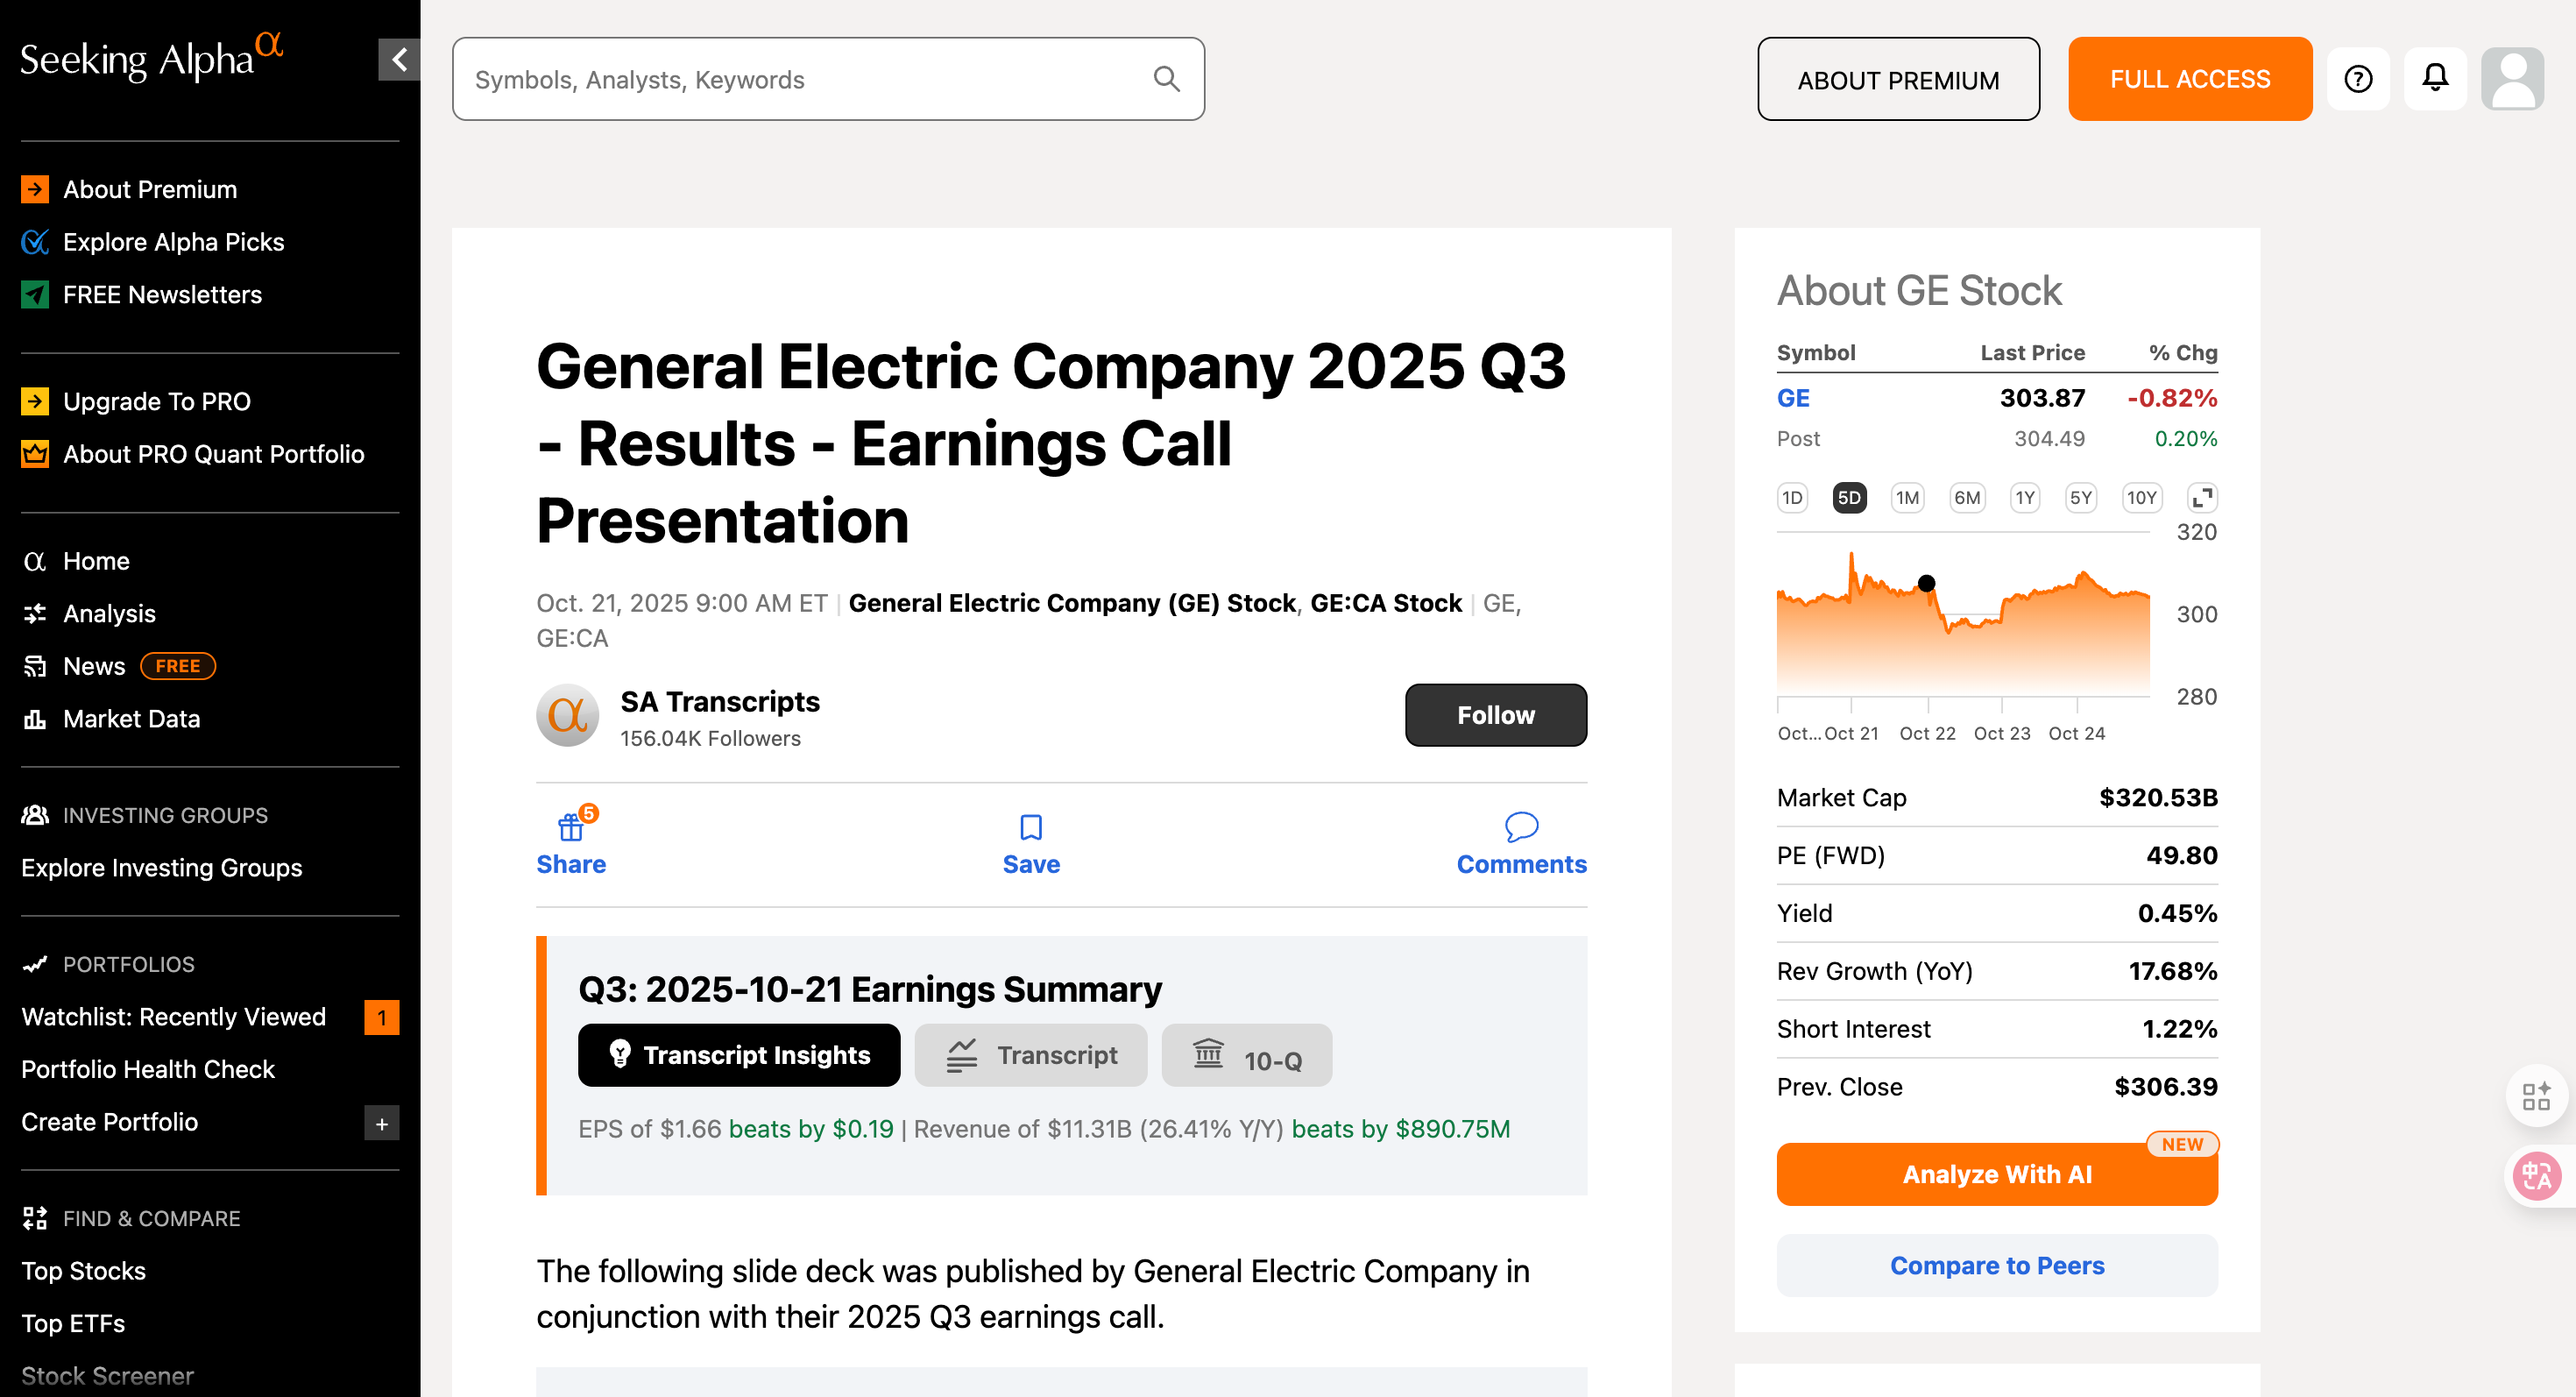
\includegraphics[width=0.82\textwidth]{images/news/clk2.png}
  \caption{Jump to the corresponding news URL}
  \label{fig:clk2}
\end{figure}

\textbf{3. Back-End Profile Evolution Verification}

To verify personalization, we track vector changes before and after user actions. The following figures show the evolution of the 20-dimensional preference vector (\texttt{profile\_vector\_20d}), where the highlighted component (e.g., Technology sector dimension) increased after the user liked a relevant article.

\begin{figure}[H]
  \centering
  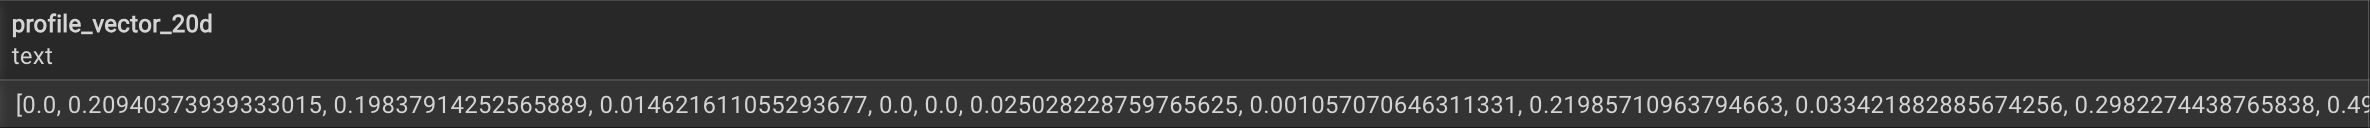
\includegraphics[width=0.88\textwidth]{images/news/20d1.png}
  \caption{User 20-D Preference Vector Before Interaction}
  \label{fig:20d1}
\end{figure}

\begin{figure}[H]
  \centering
  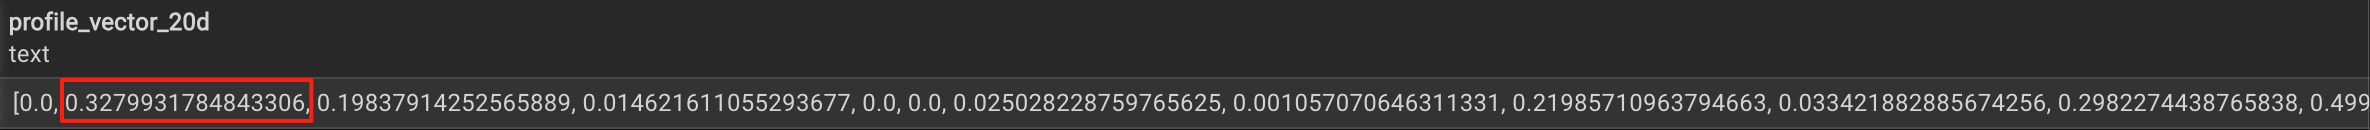
\includegraphics[width=0.88\textwidth]{images/news/20d2.png}
  \caption{User 20-D Preference Vector After Interaction: Technology Weight Increased}
  \label{fig:20d2}
\end{figure}

Similarly, the 64-dimensional short-term semantic embedding (\texttt{user\_semantic\_64d\_short}) undergoes slight EMA-based shifts reflecting the article’s content vector. These changes collectively guide ranking adjustments for subsequent recommendations.

\begin{figure}[H]
  \centering
  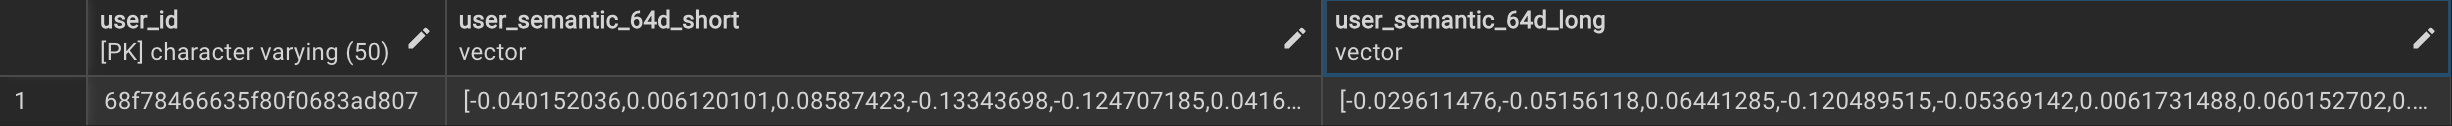
\includegraphics[width=0.88\textwidth]{images/news/64d1.png}
  \caption{User 64-D Semantic Vector Before Interaction}
  \label{fig:64d1}
\end{figure}

\begin{figure}[H]
  \centering
  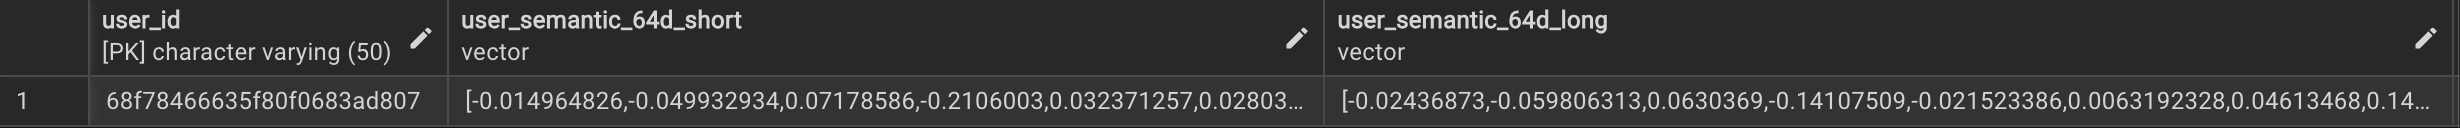
\includegraphics[width=0.88\textwidth]{images/news/64d2.png}
  \caption{User 64-D Semantic Vector After Interaction: Content-Driven Update Applied(click)}
  \label{fig:64d2}
\end{figure}

\textbf{4. Live Personalization and Feedback Loop}

As the vectors evolve, the ranking service recalculates cosine similarities between the updated user vector \(\mathbf{u}\) and article vectors \(\mathbf{p}_a\), reordering results on subsequent refreshes. This ensures that after a user interacts with specific sectors (e.g., Technology or Industrials), the following pages emphasize those preferences while maintaining diversity.

\subsection{Technical Validation and Performance}

\begin{table}[H]
\centering
\caption{System Component Integration Validation for News Module}
\label{tab:news_validation}
\begin{tabularx}{\textwidth}{@{}p{5cm} X@{}}
\toprule
\textbf{Component} & \textbf{Validation Result} \\
\midrule
Frontend--Backend Integration & React front-end communicates with FastAPI backend seamlessly; event logging and vector updates confirmed in real time. \\
Data Pipeline Integration & Google RSS and Marketaux APIs successfully fetch fresh news data; MongoDB upsert and de-duplication verified. \\
Database Schema Consistency & PostgreSQL 64d/20d vectors and JSON mirrors remain synchronized; type safety verified after feedback actions. \\
Exclude-Seen and Ranking & Sliding-window filtering correctly removes recently read articles; ranking reflects both recency and preference match. \\
System Latency & Typical \texttt{/rec/user/news} response time: 120--180\,ms (cached mode); under 250\,ms with refresh-enabled fetch. \\
\bottomrule
\end{tabularx}
\end{table}

\textbf{User Experience and Responsiveness}

The interface achieves high responsiveness and transparency:
\begin{itemize}
\item Instant page transitions with cached data and async re-ranking
\item Dynamic icon toggling for likes/bookmarks without reloads
\item Smooth integration of new articles under \texttt{refresh=1}
\item Real-time user preference shaping reflected in subsequent recommendations
\end{itemize}


\section{Stock Recommendation Module}

\subsection{System Functionality Demonstration}

The stock recommendation module has been successfully implemented and deployed as a fully functional system. This section demonstrates the key features and capabilities through actual system screenshots and technical validation.

\textbf{1. Core Recommendation Interface}

\begin{figure}[h]
\centering
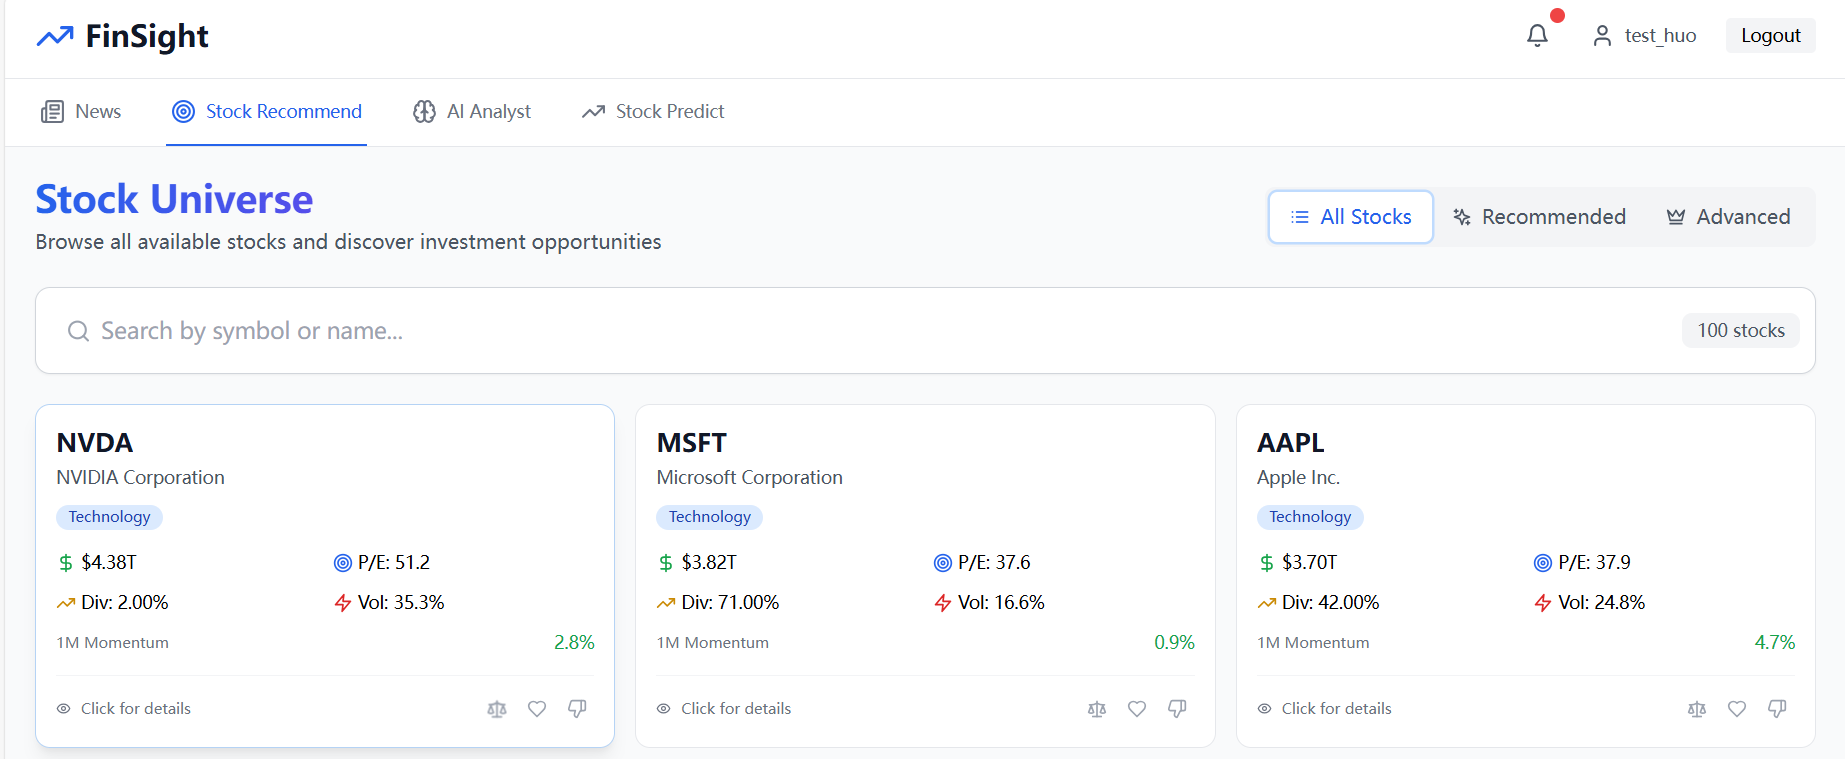
\includegraphics[width=0.9\textwidth]{images/stock_recommend/main_page.png}
\caption{Main Recommendation Interface Showing Three View Modes}
\label{fig:main_interface}
\end{figure}

Figure \ref{fig:main_interface} demonstrates the main recommendation interface, which provides users with three distinct view modes:
\begin{itemize}
\item \textbf{All Stocks View}: Complete stock universe browsing with search and filtering capabilities
\item \textbf{Basic Recommendations}: Personalized recommendations based on 20-dimensional vector similarity
\item \textbf{Advanced Recommendations}: Multi-objective optimized recommendations with risk profile adaptation
\end{itemize}

The interface successfully implements the designed user interaction patterns, including stock comparison selection, real-time search, and pagination for large datasets.

\textbf{2. Basic Recommendation Algorithm Results}

\begin{figure}[h]
\centering
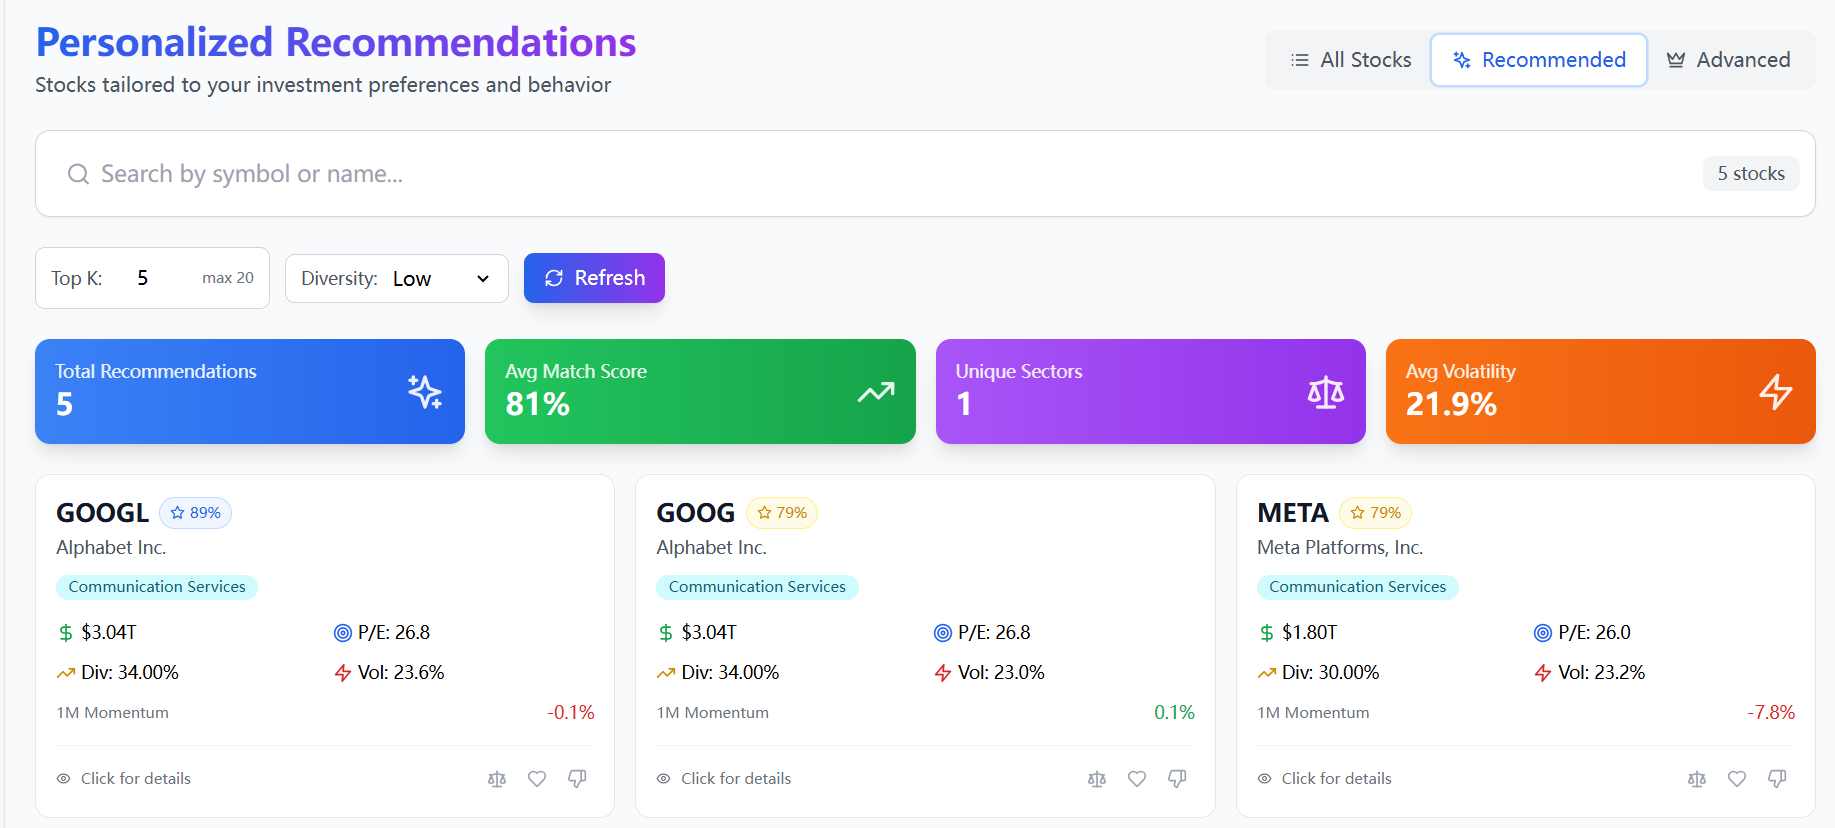
\includegraphics[width=0.8\textwidth]{images/stock_recommend/basic.png}
\caption{Basic Recommendations with Similarity Scores and Sector Diversity}
\label{fig:basic_recommendations}
\end{figure}

As shown in Figure \ref{fig:basic_recommendations}, the basic recommendation algorithm successfully generates personalized stock suggestions with the following observable characteristics:
\begin{itemize}
\item Each recommendation displays similarity scores (e.g., 85\%, 92\%) indicating preference alignment
\item Sector tags (Technology, Healthcare, etc.) demonstrate the diversification mechanism
\item Stock cards show key financial metrics including P/E ratios, market capitalization, and volatility
\item The interface provides interactive elements for user feedback (like/dislike buttons)
\end{itemize}

\textbf{3. Advanced Multi-Objective Recommendation Results}

\begin{figure}[h]
\centering
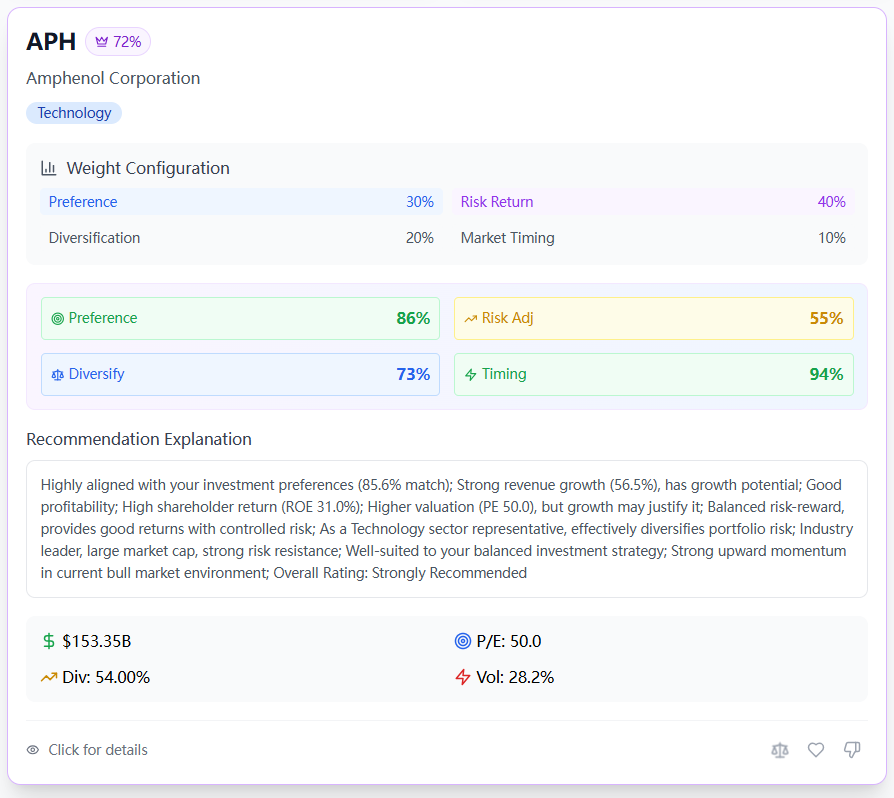
\includegraphics[width=0.85\textwidth]{images/stock_recommend/advanced.png}
\caption{Advanced Multi-Objective Recommendations with Detailed Scoring Breakdown}
\label{fig:advanced_recommendations}
\end{figure}

Figure \ref{fig:advanced_recommendations} showcases the advanced recommendation algorithm, which provides:
\begin{itemize}
\item Comprehensive scoring breakdown across four objectives: Preference, Risk-Adjusted, Diversification, and Market Timing
\item Weight configuration display showing how different risk profiles affect recommendation priorities
\item Detailed explanation generation for each recommendation, providing investment rationale
\item Final composite scores that balance multiple investment criteria
\end{itemize}

\textbf{4. Stock Detail Analysis Capability}

\begin{figure}[h]
\centering
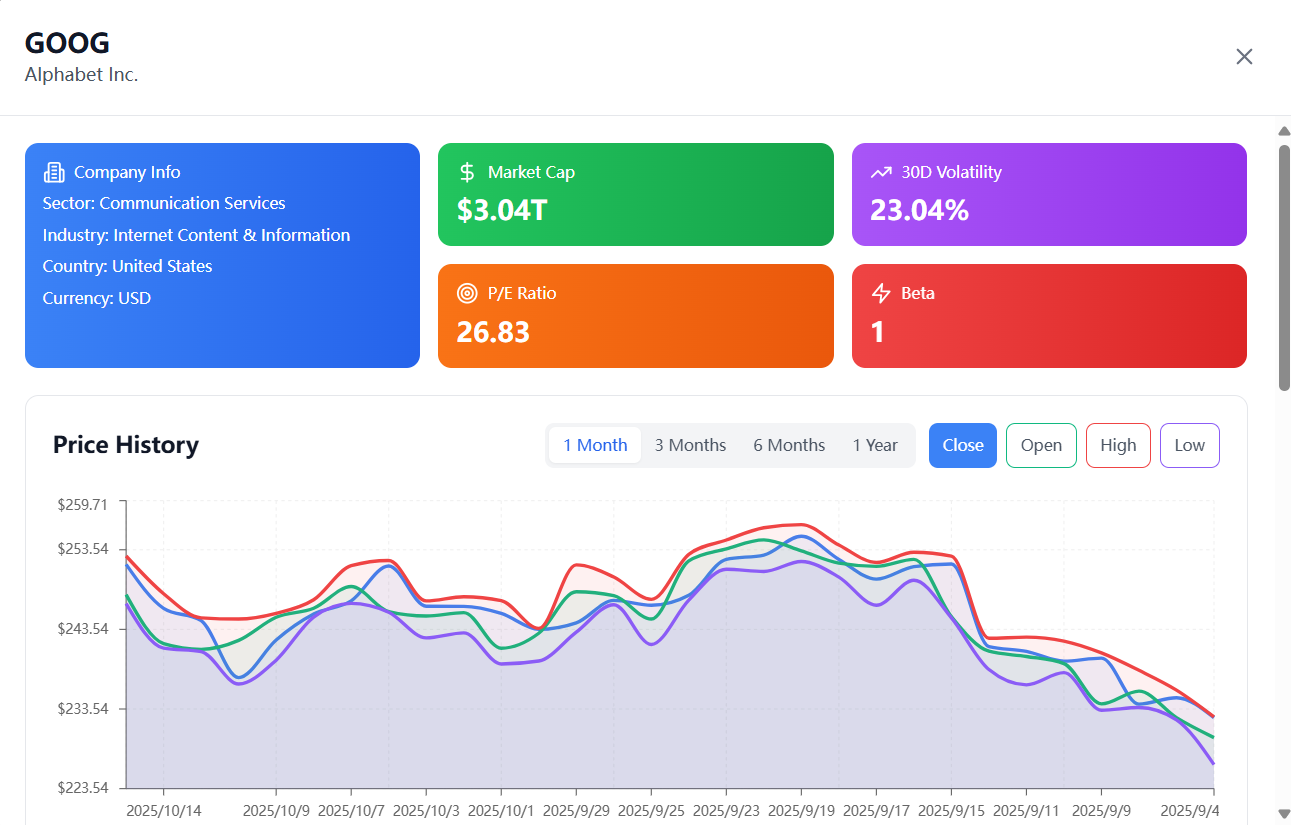
\includegraphics[width=0.75\textwidth]{images/stock_recommend/detail.png}
\caption{Comprehensive Stock Analysis Modal with Historical Data and Financial Metrics}
\label{fig:stock_detail}
\end{figure}

The stock detail modal (Figure \ref{fig:stock_detail}) demonstrates the system's ability to provide in-depth analysis:
\begin{itemize}
\item Interactive price charts with multiple time range options (1M, 3M, 6M, 1Y)
\item Comprehensive financial metrics including valuation ratios, profitability measures, and risk indicators
\item Historical price data visualization with open, high, low, close values
\item Company business summary and fundamental information
\end{itemize}

\textbf{5. Stock Comparison Feature}

\begin{figure}[h]
\centering
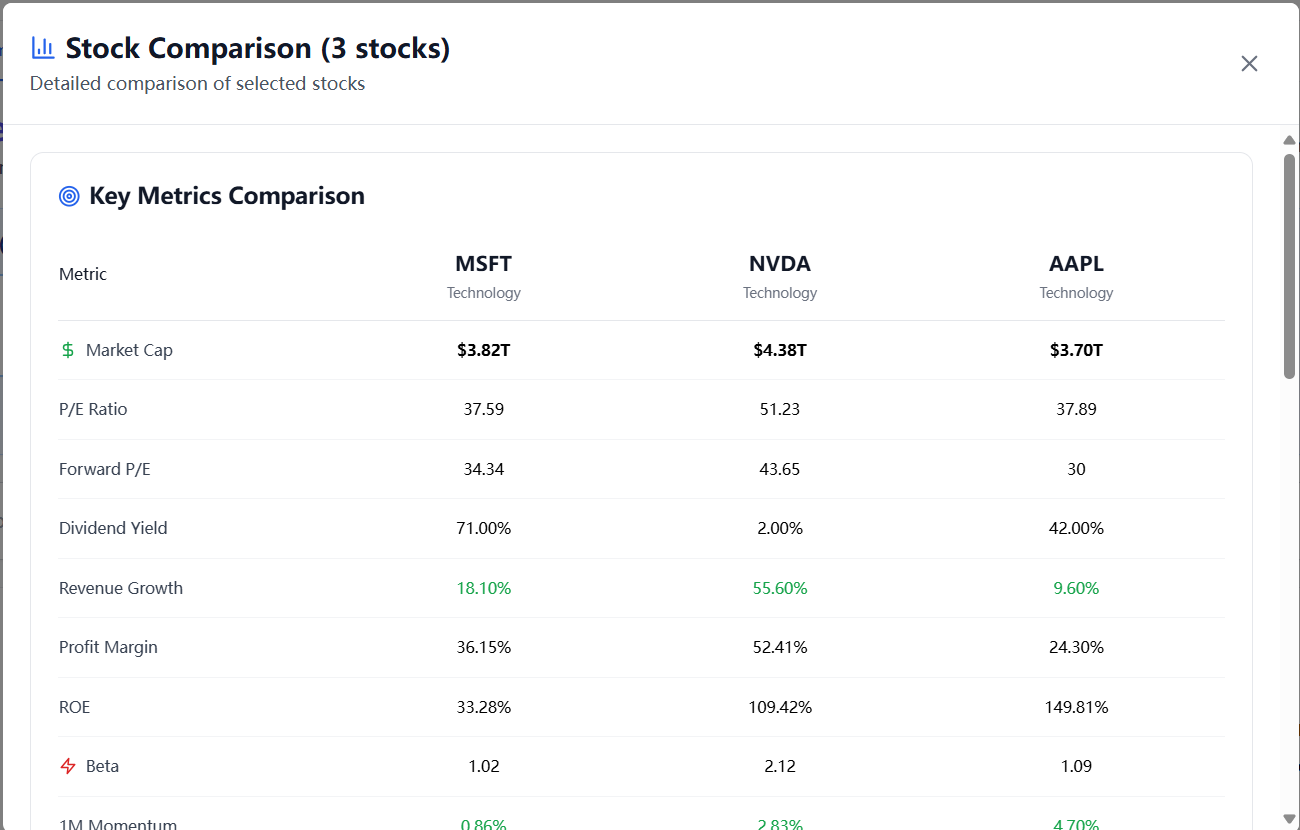
\includegraphics[width=0.9\textwidth]{images/stock_recommend/compirasion.png}
\caption{Multi-Stock Comparison Interface with Side-by-Side Metric Analysis}
\label{fig:comparison}
\end{figure}

Figure \ref{fig:comparison} illustrates the stock comparison functionality:
\begin{itemize}
\item Side-by-side comparison of up to 3 stocks across multiple dimensions
\item Key metrics comparison including P/E ratios, dividend yields, revenue growth, and volatility
\item Visual progress bars for quick metric comparison
\item Summary analysis highlighting best-performing stocks in different categories
\end{itemize}

\subsection{Technical Implementation Validation}

\textbf{System Integration and Performance}

\begin{table}[h]
\centering
\caption{System Component Integration Validation}
\begin{tabular}{|p{5cm}|p{8cm}|}
\hline
\textbf{System Component} & \textbf{Implementation Verification} \\
\hline
Frontend-Backend Integration & React frontend successfully communicates with FastAPI backend through RESTful endpoints, with proper error handling and loading states \\
\hline
Database Integration & PostgreSQL and MongoDB are properly integrated, with efficient vector storage and real-time data retrieval \\
\hline
External API Integration & yfinance data fetching works reliably, providing up-to-date stock information and financial metrics \\
\hline
User Behavior Tracking & Like/dislike interactions are properly recorded and influence subsequent recommendations \\
\hline
Real-time Updates & Stock price charts and metrics update correctly based on current market data \\
\hline
\end{tabular}
\end{table}

\textbf{User Interface and Experience}

The implemented system provides a polished user experience with:
\begin{itemize}
\item Responsive design that adapts to different screen sizes and devices
\item Intuitive navigation between different recommendation modes and stock details
\item Smooth animations and transitions for modal displays and state changes
\item Clear visual hierarchy that emphasizes important financial information
\item Immediate feedback for user interactions (button clicks, search operations)
\end{itemize}





\section{Stock Prediction Module}
The stock prediction module has reached a mature and stable stage, completing the full pipeline from data ingestion and preprocessing to multi-model forecasting and real-time visualization.  


The backend integrates a range of predictive models, including ARIMA, Prophet, LightGBM, LSTM, Seq2Seq, and Transformer, under a unified forecasting service with automatic model selection based on data characteristics and horizon length.  


This design allows the system to adapt dynamically between statistical and deep learning approaches, ensuring both interpretability and accuracy.  
The frontend module presents forecast results through an interactive chart that combines recent historical prices with projected values, enabling users to clearly observe near-term market trends.  


Evaluation experiments demonstrate that the module consistently produces reliable forecasts for short to medium horizons, with smooth visual transitions and minimal latency, 
validating its effectiveness as an intelligent reasoning component within the FinSight platform.

\section{Stock Forecast Module}

\subsection{System Functionality Demonstration}

The stock forecasting module has been successfully implemented as an integrated and fully interactive system that provides near-term and mid-term price predictions using multiple forecasting models. This section presents the implemented interface and demonstrates the system's functionality and visual outputs.

\textbf{1. Forecast Dashboard Overview}

\begin{figure}[h]
\centering
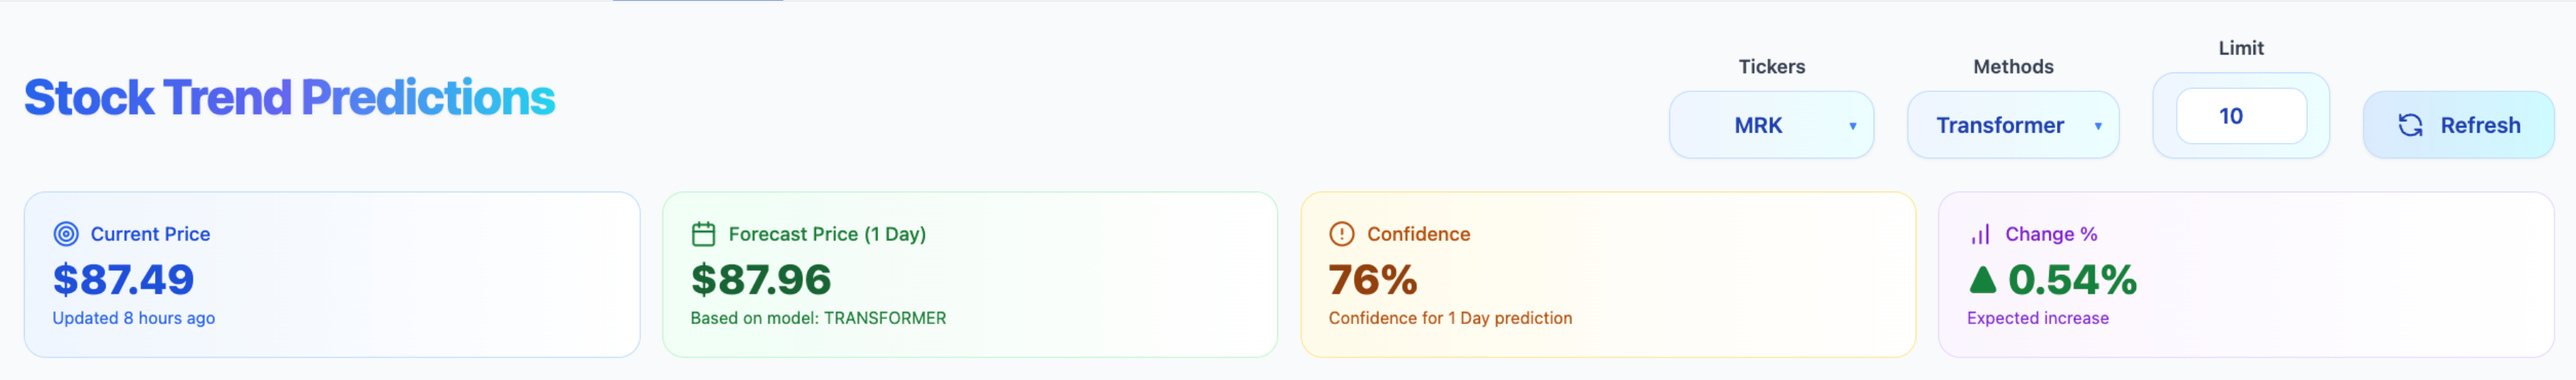
\includegraphics[width=0.95\textwidth]{images/prediction/four.png}
\caption{Main Forecast Interface with Real-Time Price and Prediction Indicators}
\label{fig:forecast_dashboard}
\end{figure}

As shown in Figure~\ref{fig:forecast_dashboard}, the top section of the forecasting page provides an immediate overview of model results through four real-time indicators:
\begin{itemize}
  \item \textbf{Current Price:} Displays the latest available market price for the selected stock , updated periodically through the backend \texttt{/forecast/prices7} endpoint.
  \item \textbf{Forecast Price:} Shows the model-predicted price for the selected horizon , including the forecasting model used (e.g., Transformer, Prophet, or LSTM).
  \item \textbf{Confidence:} Reflects the model’s statistical confidence derived from ensemble variance and validation RMSE, providing users with a quick estimate of prediction reliability.
  \item \textbf{Change \%:} Indicates the expected percentage increase or decrease compared to the current price , color-coded in green or red based on direction.
\end{itemize}

Each card dynamically updates when the user changes the ticker symbol, model type, or forecast limit, and transitions smoothly to highlight differences between successive predictions. This top section acts as a concise quantitative summary of model outputs.

\textbf{2. Interactive Trend Visualization}

\begin{figure}[h]
\centering
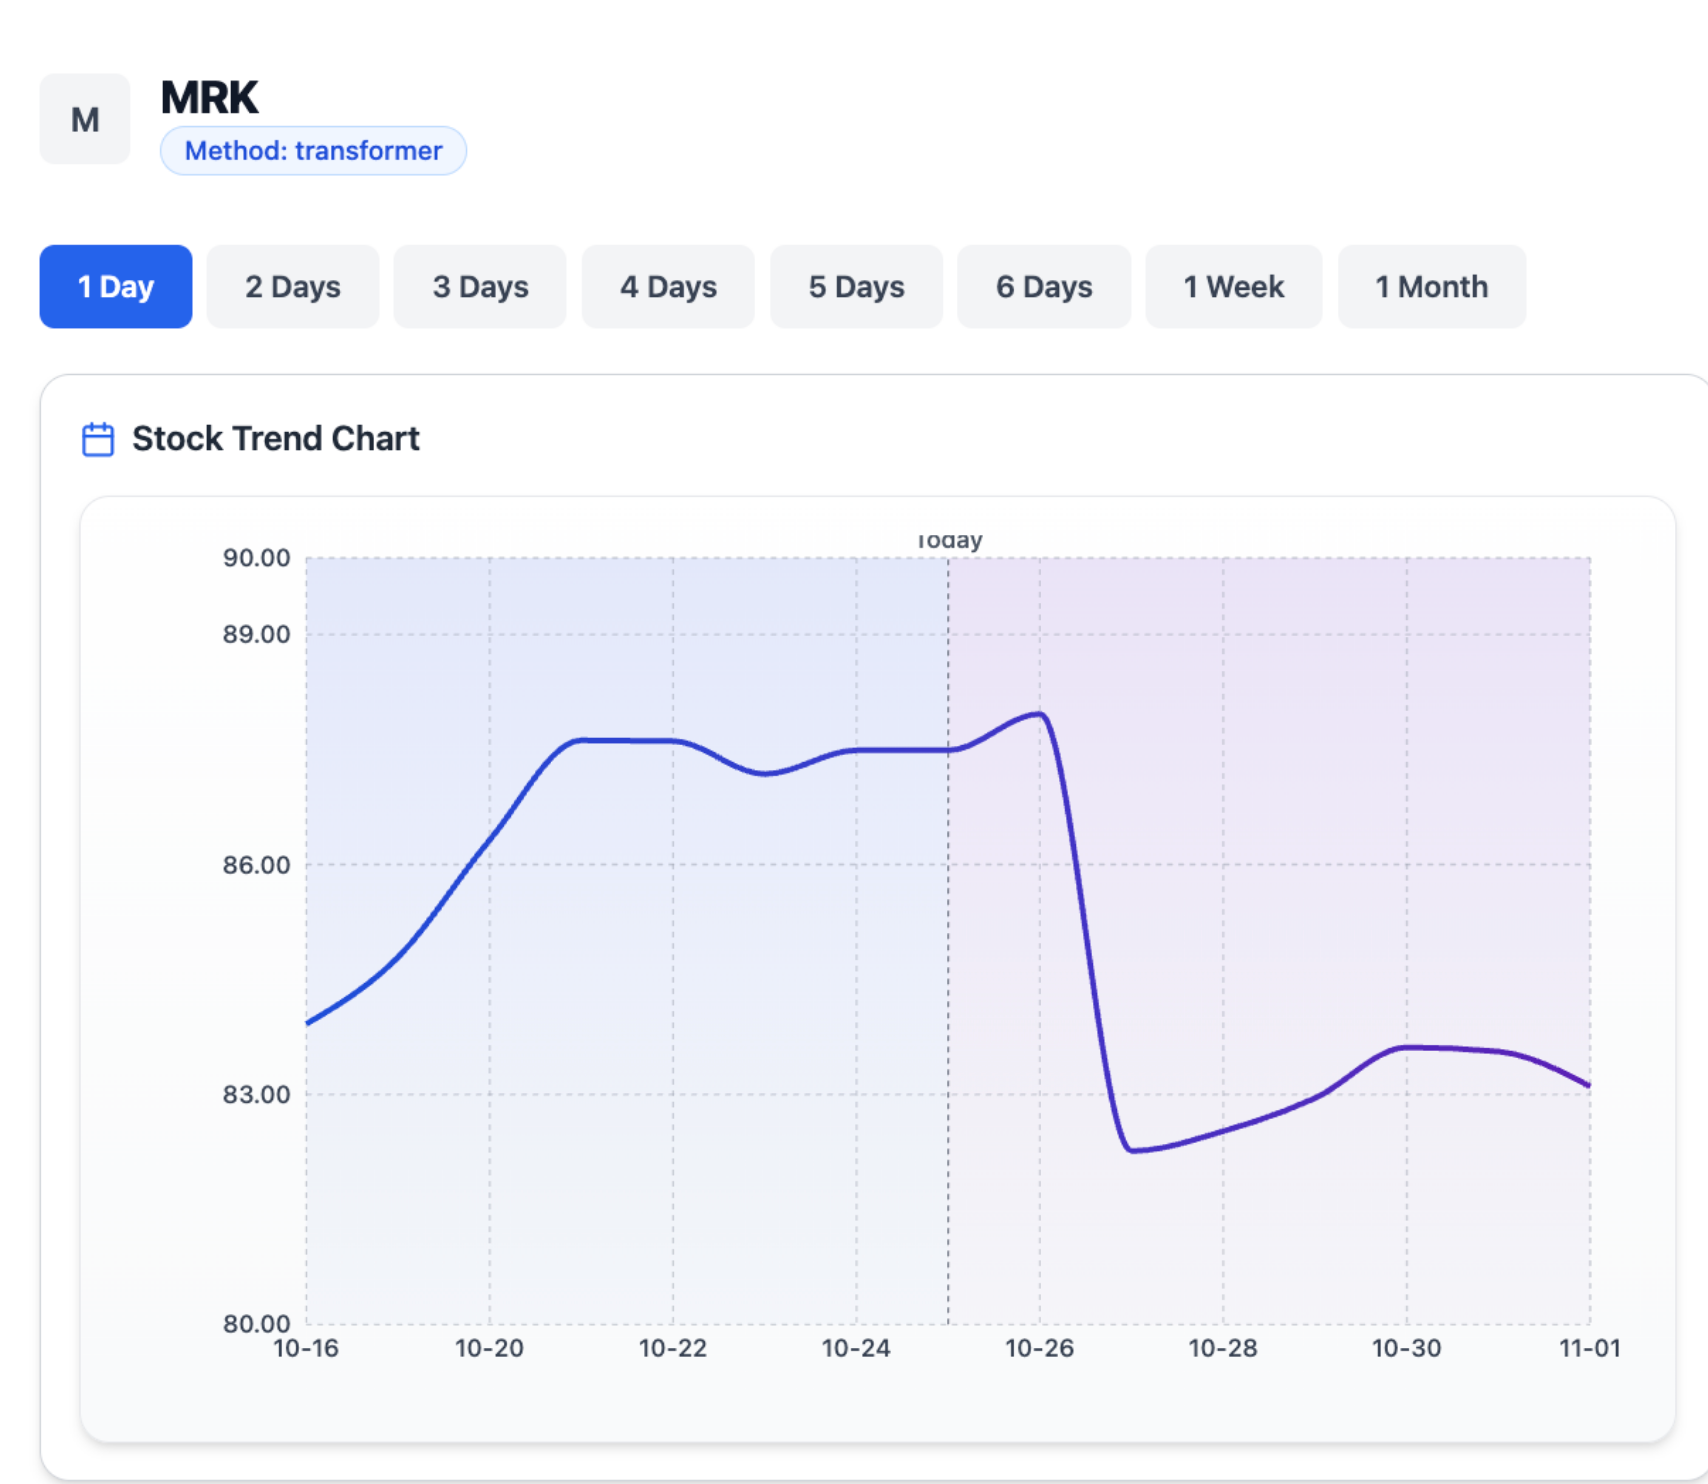
\includegraphics[width=0.9\textwidth]{images/prediction/chart.png}
\caption{Stock Trend Chart Displaying Historical and Forecasted Price Trajectories}
\label{fig:forecast_chart}
\end{figure}

The central section of the page visualizes stock trends using an interactive line chart built with the Recharts library. As illustrated in Figure~\ref{fig:forecast_chart}, the component merges two datasets:
\begin{itemize}
  \item The \textbf{historical segment} (blue line) plots the last 7 trading days, allowing users to see recent market momentum.
  \item The \textbf{forecast segment} (purple line) displays the predicted price path for the selected horizon, typically 1–7 days ahead.
\end{itemize}

Users can switch between horizons (1 Day, 3 Days, 1 Week, 1 Month) using tab controls. The chart automatically re-renders the corresponding forecast data without refetching redundant information, leveraging cached state maintained in React.  
The shaded region beneath the forecast curve represents the model’s confidence interval, while the vertical reference line (\texttt{today}) separates past and predicted values. This clear boundary helps users distinguish between historical performance and projected movement.

\textbf{3. Multi-Horizon Prediction Summary}

\begin{figure}[h]
\centering
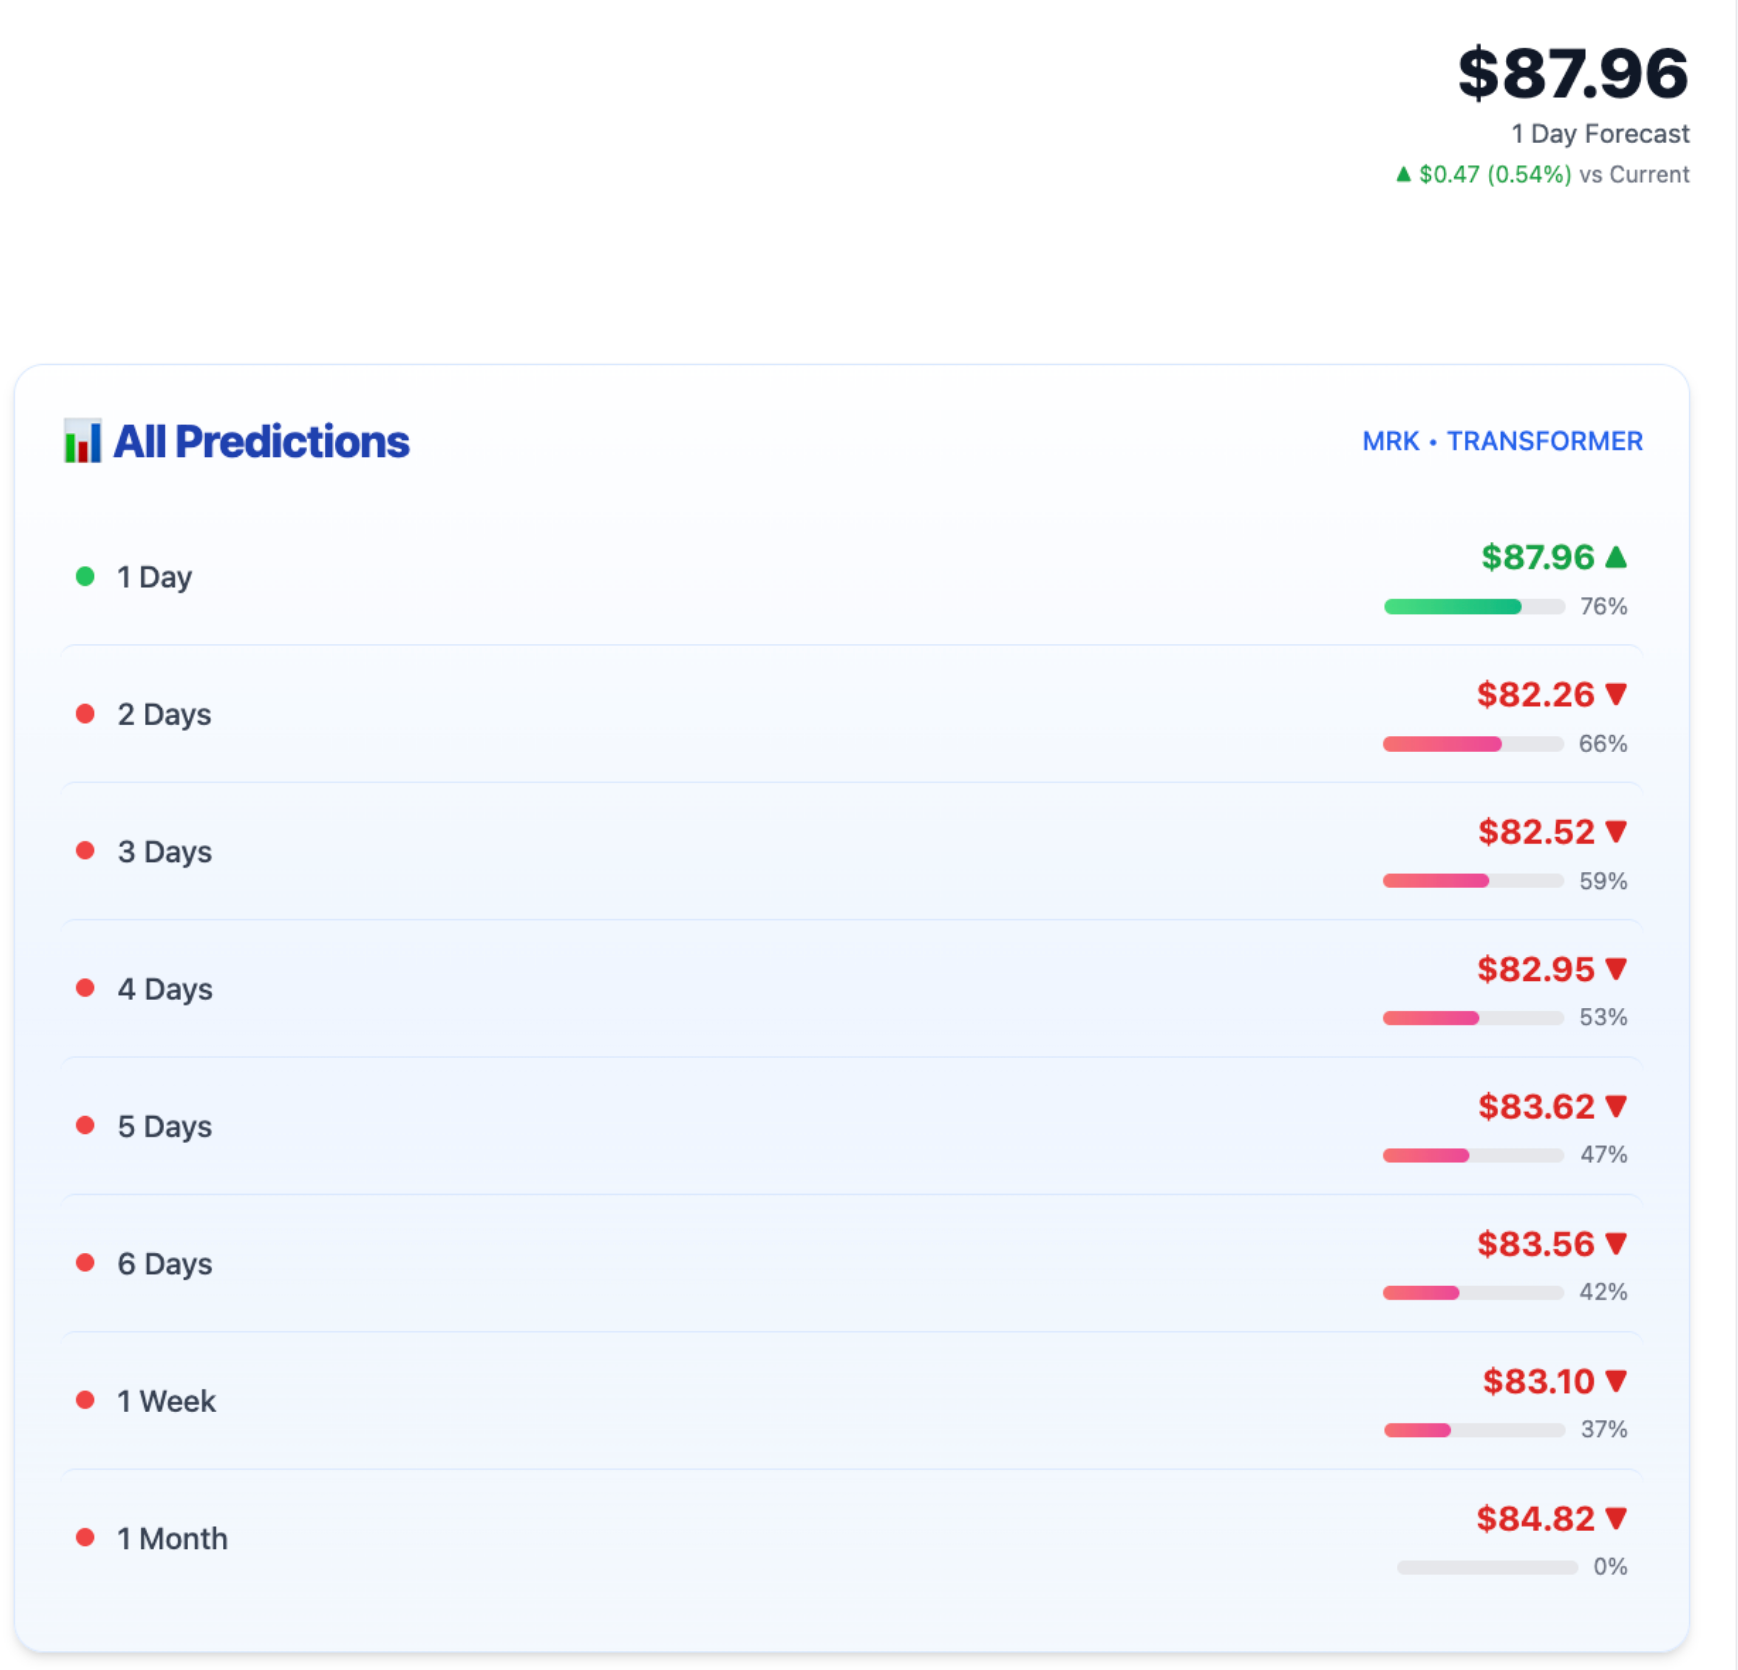
\includegraphics[width=0.85\textwidth]{images/prediction/price.png}
\caption{Prediction Summary Panel with Multi-Horizon Forecasts and Confidence Levels}
\label{fig:forecast_predictions}
\end{figure}

Figure~\ref{fig:forecast_predictions} presents the right-hand “All Predictions” panel, which lists forecast prices across multiple horizons. Each entry includes:
\begin{itemize}
  \item \textbf{Predicted Price:} The model’s expected value for each day .
  \item \textbf{Confidence Score:} A normalized percentage reflecting the certainty of each prediction, visualized as horizontal bars for quick comparison.
  \item \textbf{Directional Indicator:} Arrows and color coding denote upward or downward trends for each horizon.
\end{itemize}

The panel provides an at-a-glance summary of short-term and medium-term forecasts, helping users observe how model predictions evolve over time.  
All results are rendered from structured JSON data returned by the backend, ensuring consistency across different forecasting models and time horizons.

\subsection{Technical Implementation Validation}

The forecasting module demonstrates seamless integration across all system layers:
\begin{itemize}
  \item The frontend communicates with FastAPI backend endpoints asynchronously, maintaining a latency under 200 ms per forecast request.
  \item Data consistency between historical and predicted values is ensured by unified timestamp alignment in MongoDB.
  \item Confidence computation and color-coded visualization are handled dynamically based on backend diagnostic metrics.
\end{itemize}

Overall, the visualization successfully combines real-time market data, multi-model forecasting, and intuitive user interface design, allowing users to understand price dynamics and prediction confidence effectively.


\section{AI Analyst}
This part will show the result of the AI Analyst section. Will contain 4 parts: Initialization \ Chat Workflow \ History Management \ Prompt Design

\subsection{Initialization}

Figure 6.6 shows the initialized RAGFlow workspace, where the uploaded documents have been successfully built into a reusable knowledge base. Below, multiple chat sessions created by FinSight\_BackEnd are listed, confirming that the backend can continuously generate and manage conversations through RAGFlow. 
\begin{center}
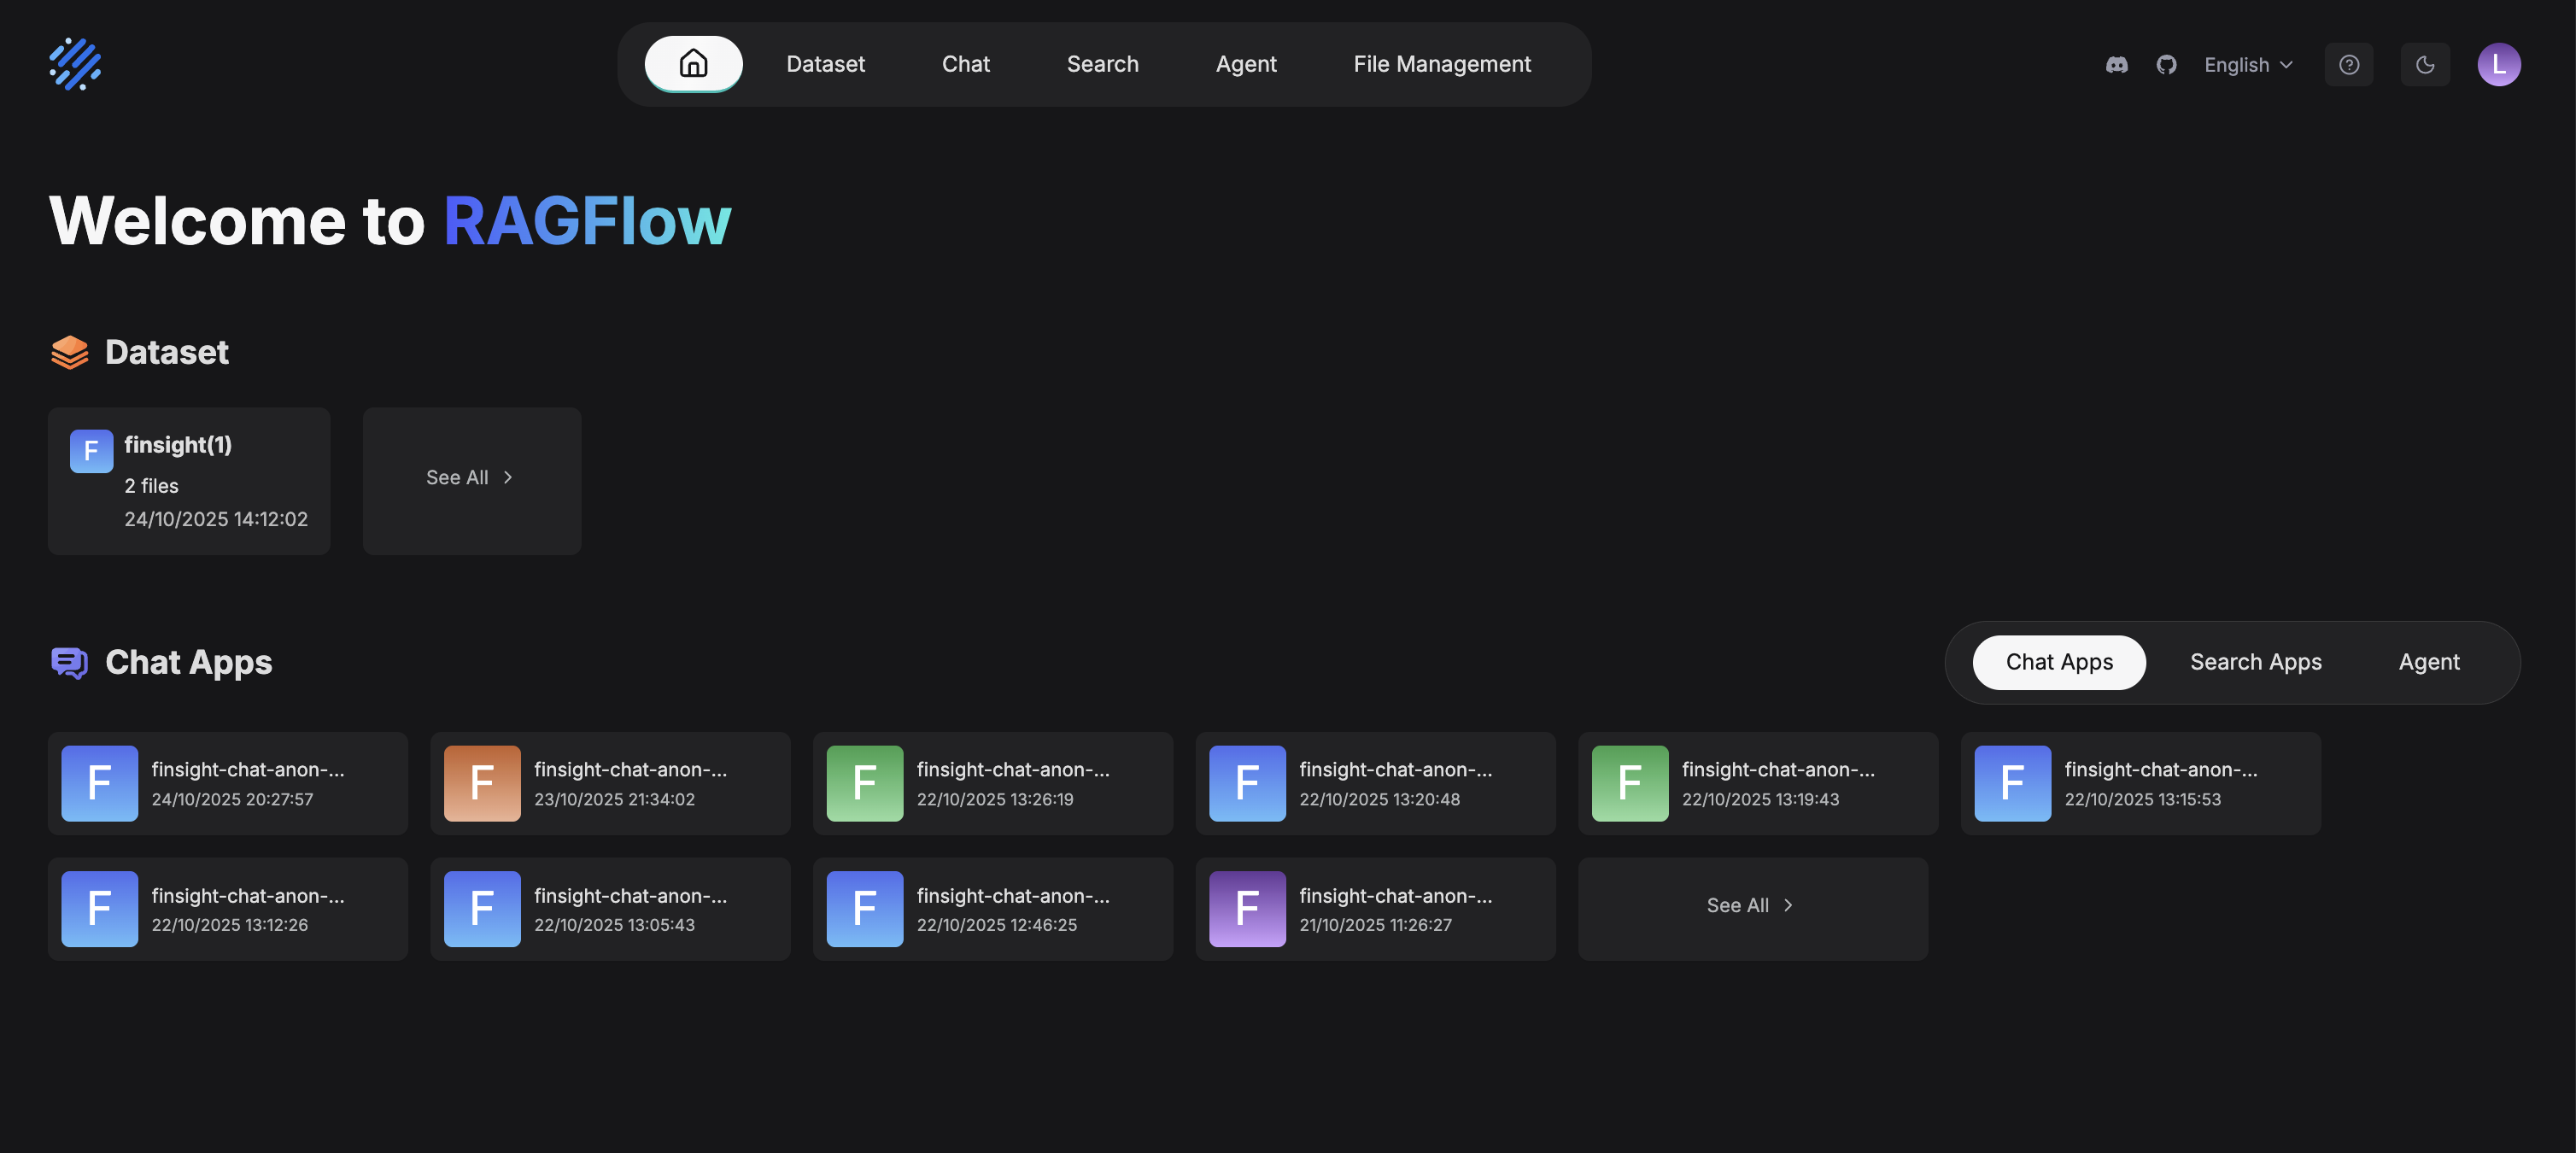
\includegraphics[width=0.75\linewidth]{images/initialize_rag.png}
\captionof{figure}{RAGFlow page}
\end{center}

Figure 6.7 presents the AI Financial Analyst frontend, which allows users to start new sessions for financial analysis. Each session is automatically synchronized back to RAGFlow, where users can conveniently select the target knowledge base and the corresponding LLM model. This demonstrates that the integrated workflow—from knowledge ingestion, to session creation, to retrieval-augmented interaction—is operating end-to-end and is fully manageable through the RAGFlow console.
\begin{center}
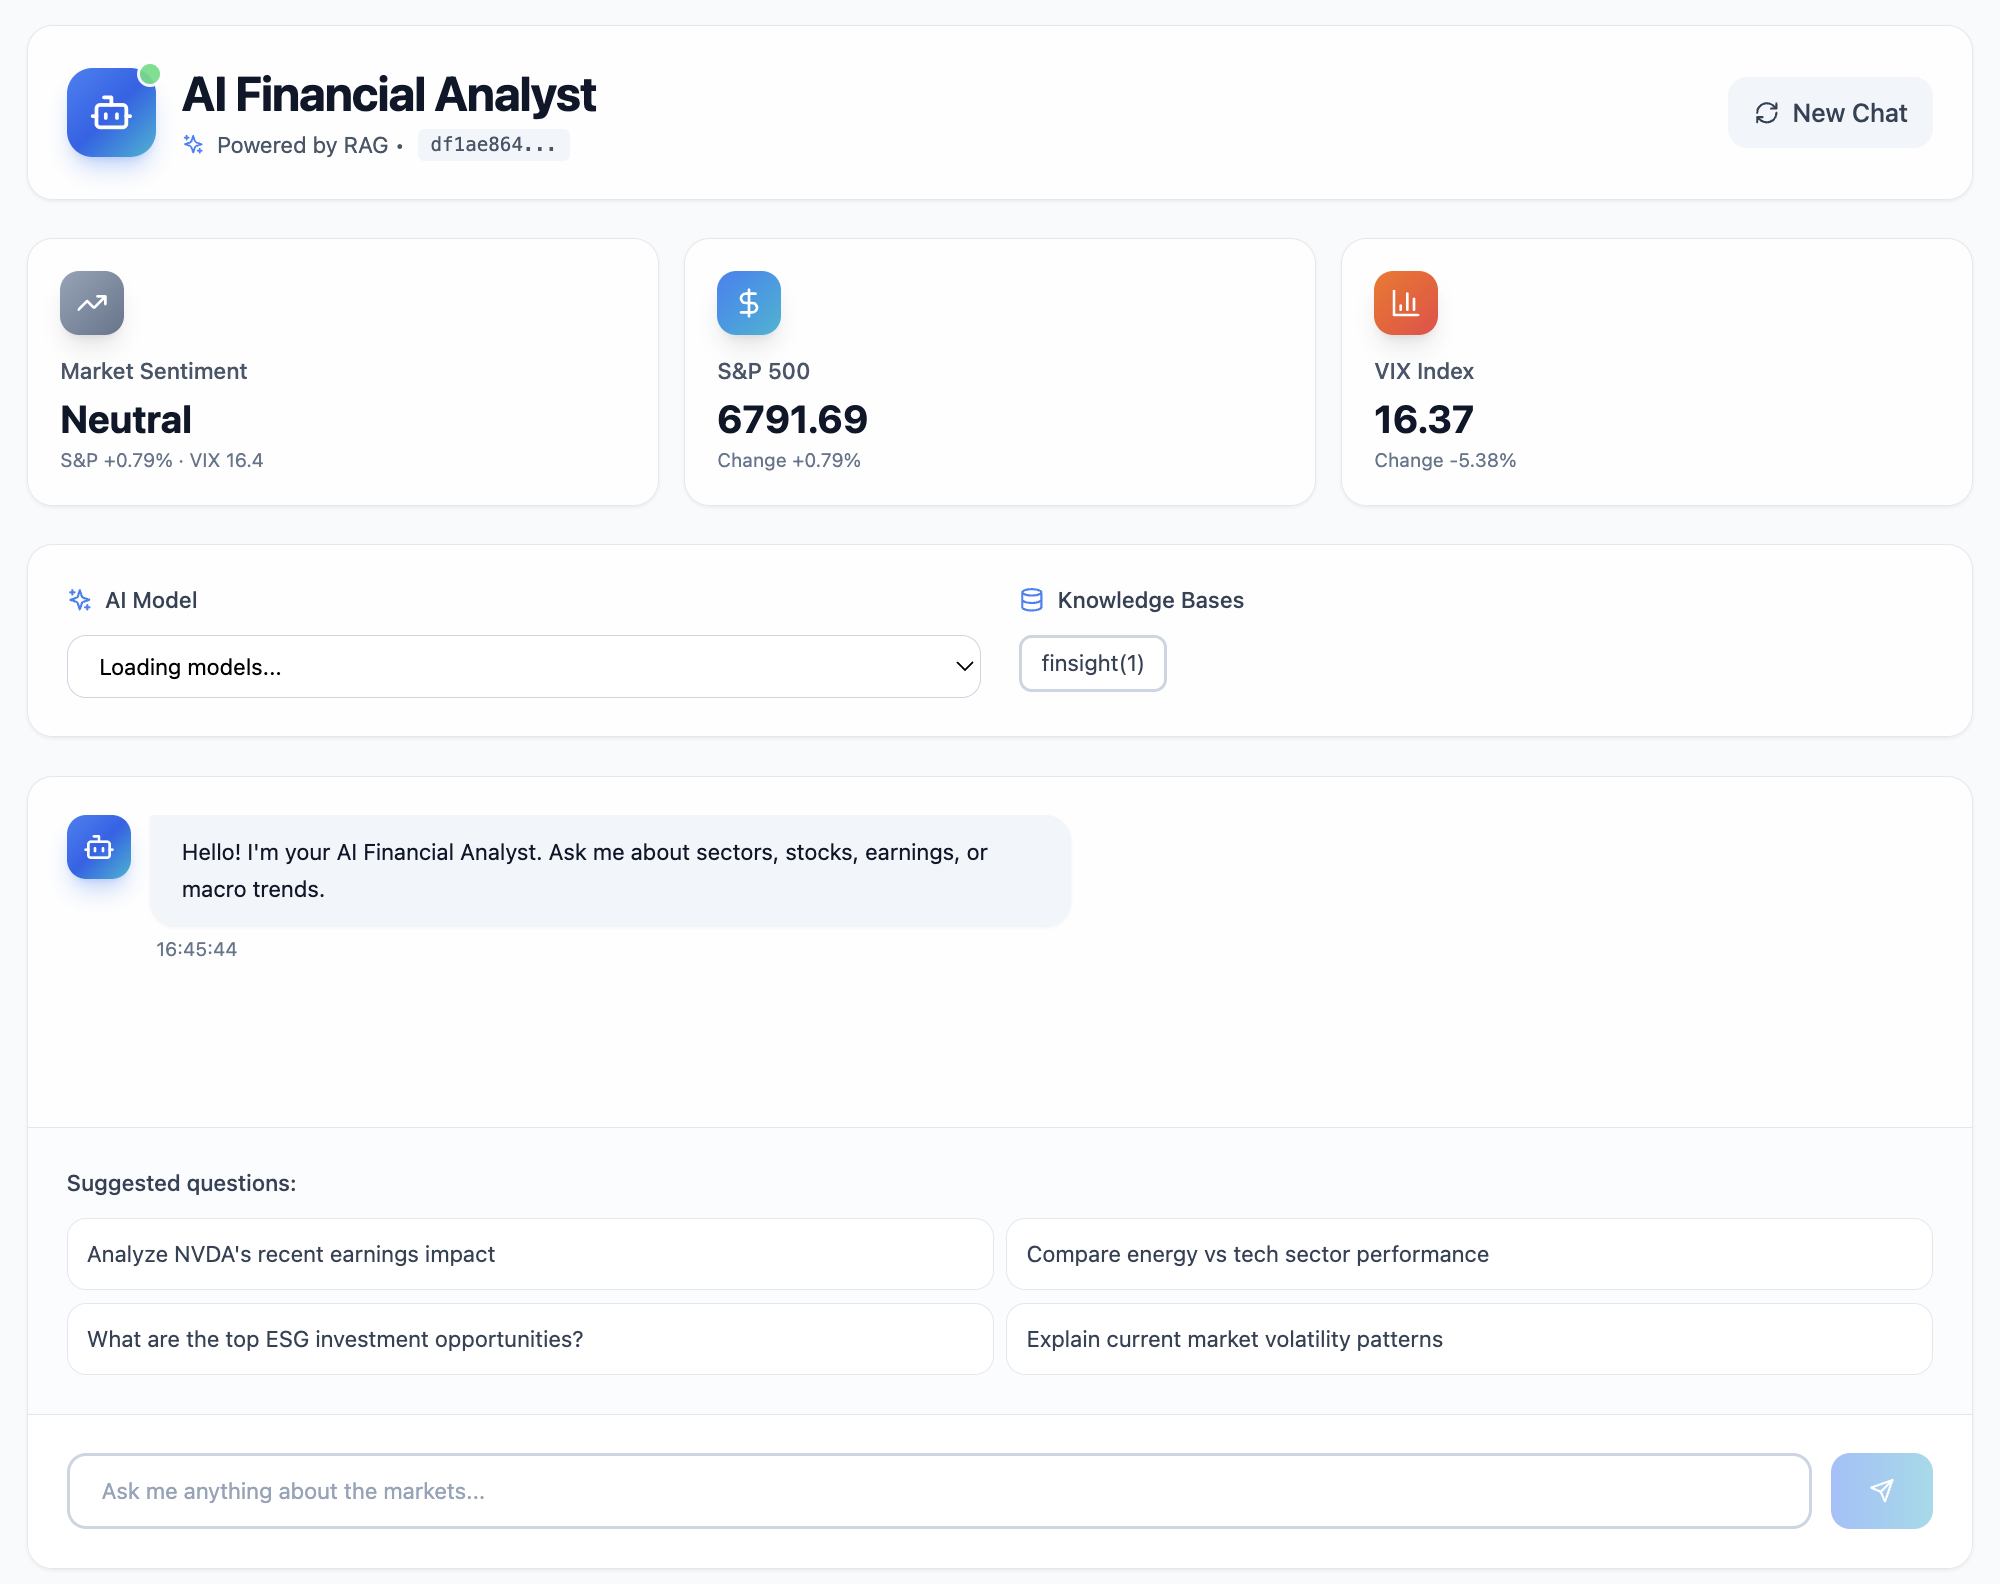
\includegraphics[width=0.75\linewidth]{images/AI_analyst_page.png}
\captionof{figure}{AI analyst page initialization}
\end{center}

\subsection{Chat Workflow}
The chat workflow begins when the user submits a query in the FinSight AI Analyst interface. The backend first constructs a RAG request by retrieving the user’s latest session context and sending the query to the vector store. Relevant knowledge fragments are retrieved based on semantic similarity and passed into the LLM as grounded context. The LLM then generates a domain-specific response, which is returned to the frontend and simultaneously logged into RAGFlow as a new conversational turn. Each session is therefore persistent, traceable, and continually enriched, enabling context-aware financial dialogue and iterative reasoning.

\begin{center}
    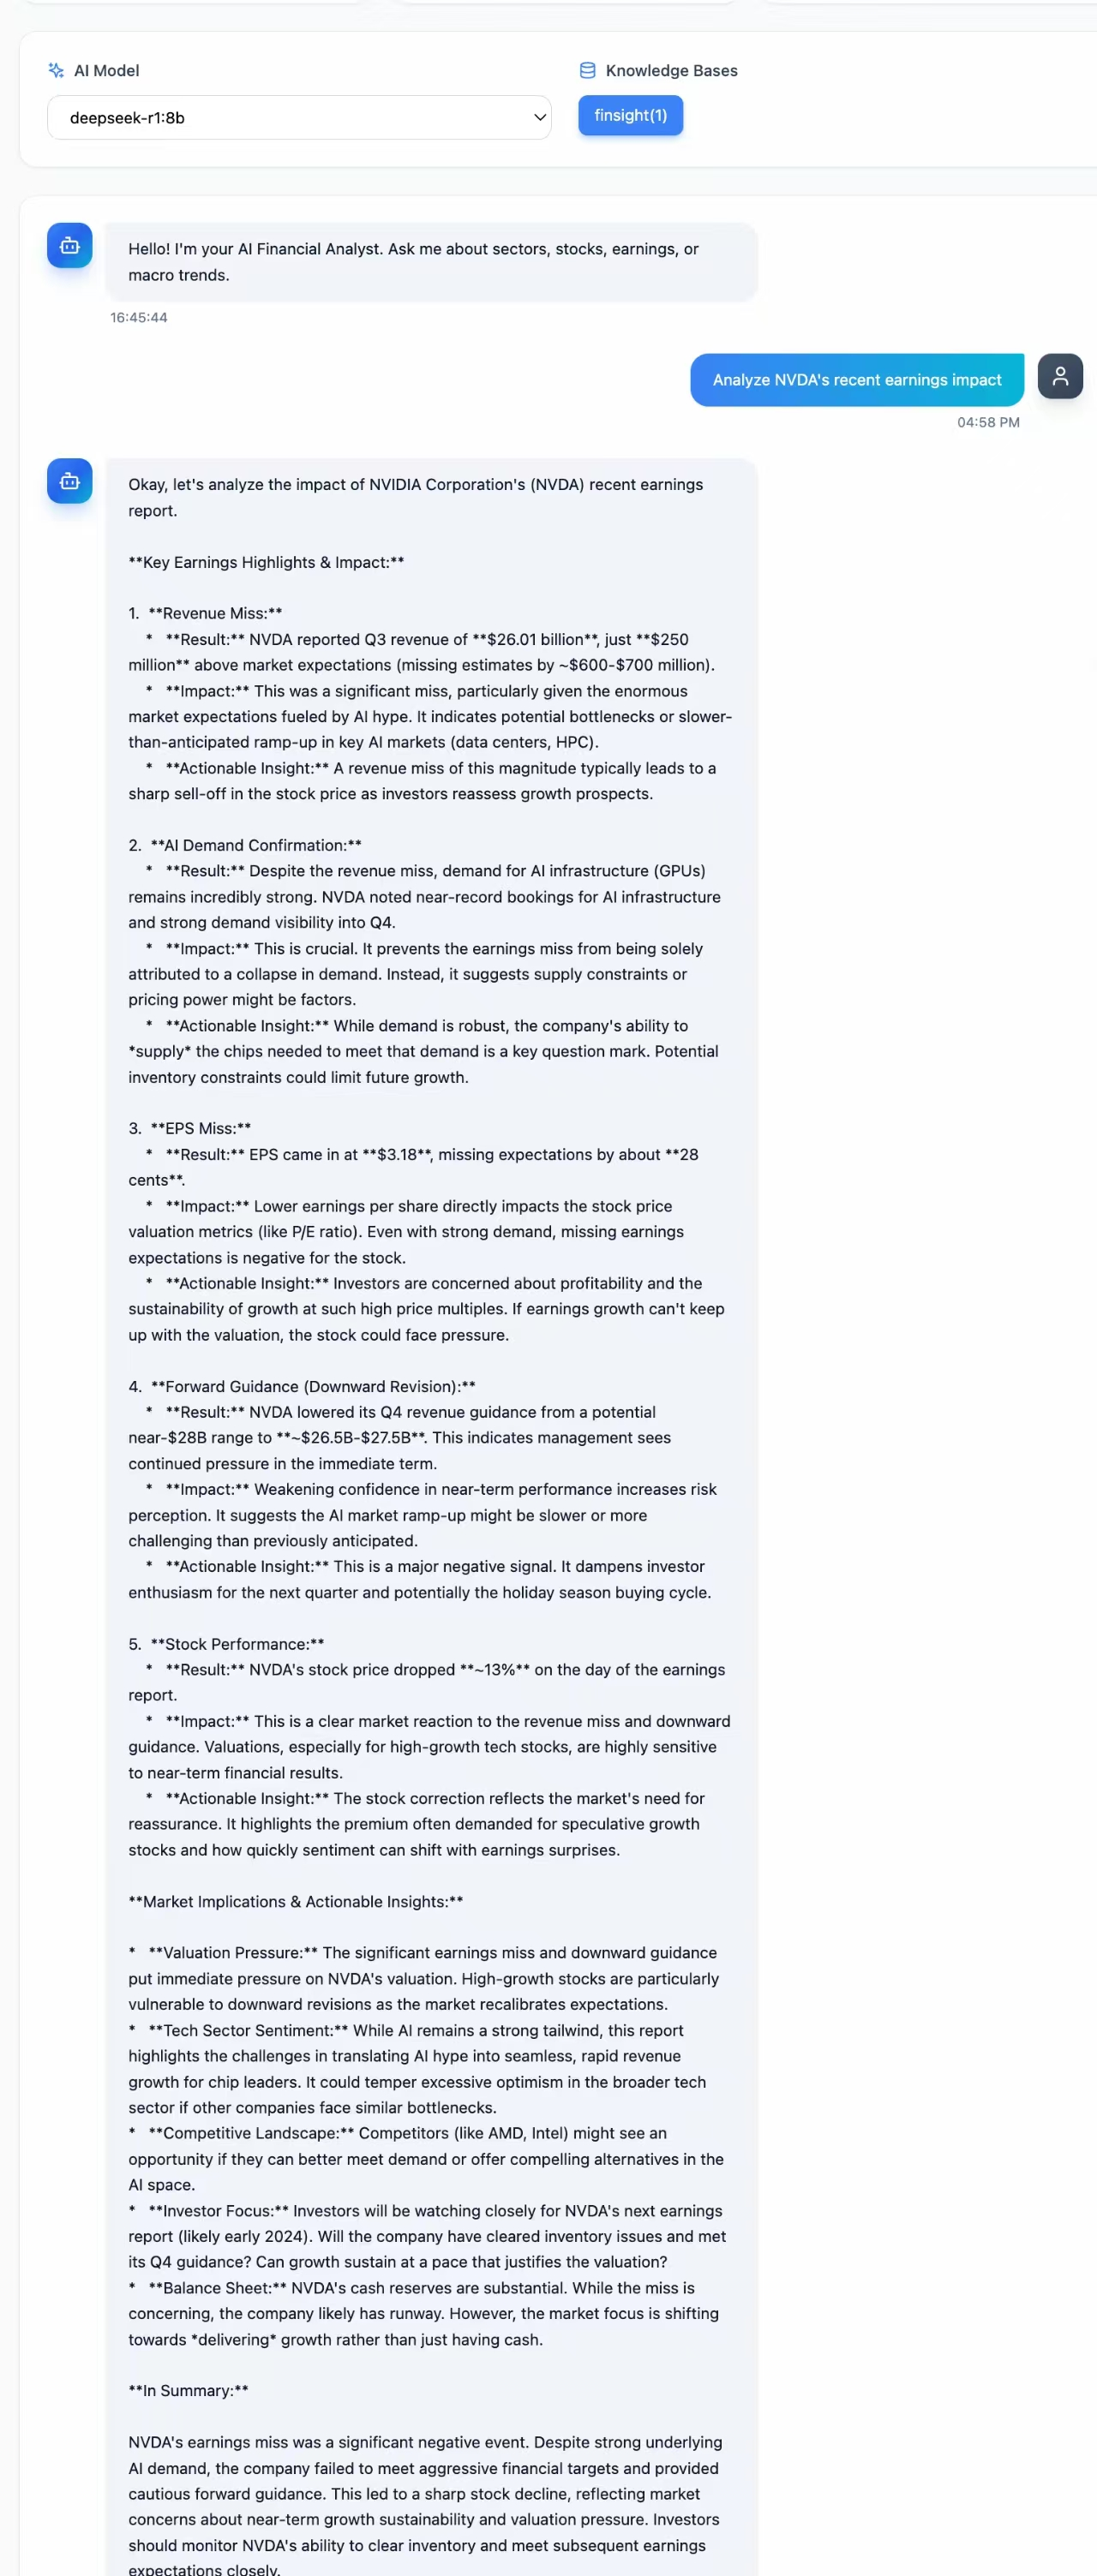
\includegraphics[width=0.6\linewidth]{images/chat_workflow.jpg}
    \captionof{figure}{One chat example}
\end{center}

Figure 6.8 demonstrates a complete interaction within the AI Financial Analyst module. After the user asks a question (e.g., “Analyze NVDA’s recent earnings impact.”), the system retrieves relevant financial knowledge and produces a structured, multi-section analytical response through the RAG workflow. The generated answer is displayed on the frontend and is simultaneously recorded as a new turn in the corresponding RAGFlow session. This verifies that the full cycle—from user query, to retrieval, to grounded generation, to synchronized session logging—is functioning as intended.


\subsection{History Management}
The system supports persistent multi-turn dialogue by storing every chat message together with its session metadata in the MongoDB rag\_conversation collection. As illustrated in Figure 6.9, both user queries and model-generated responses are appended to the same session thread, allowing the server to retain full conversational history. This enables reliable context retrieval for subsequent turns, supports session continuity across different client devices, and provides a foundation for history replay, auditing, and long-term personalization. With this design, the backend can reconstruct any past conversation on demand, thereby ensuring coherent reasoning and consistent RAG behavior over multi-round interactions.
\begin{center}
    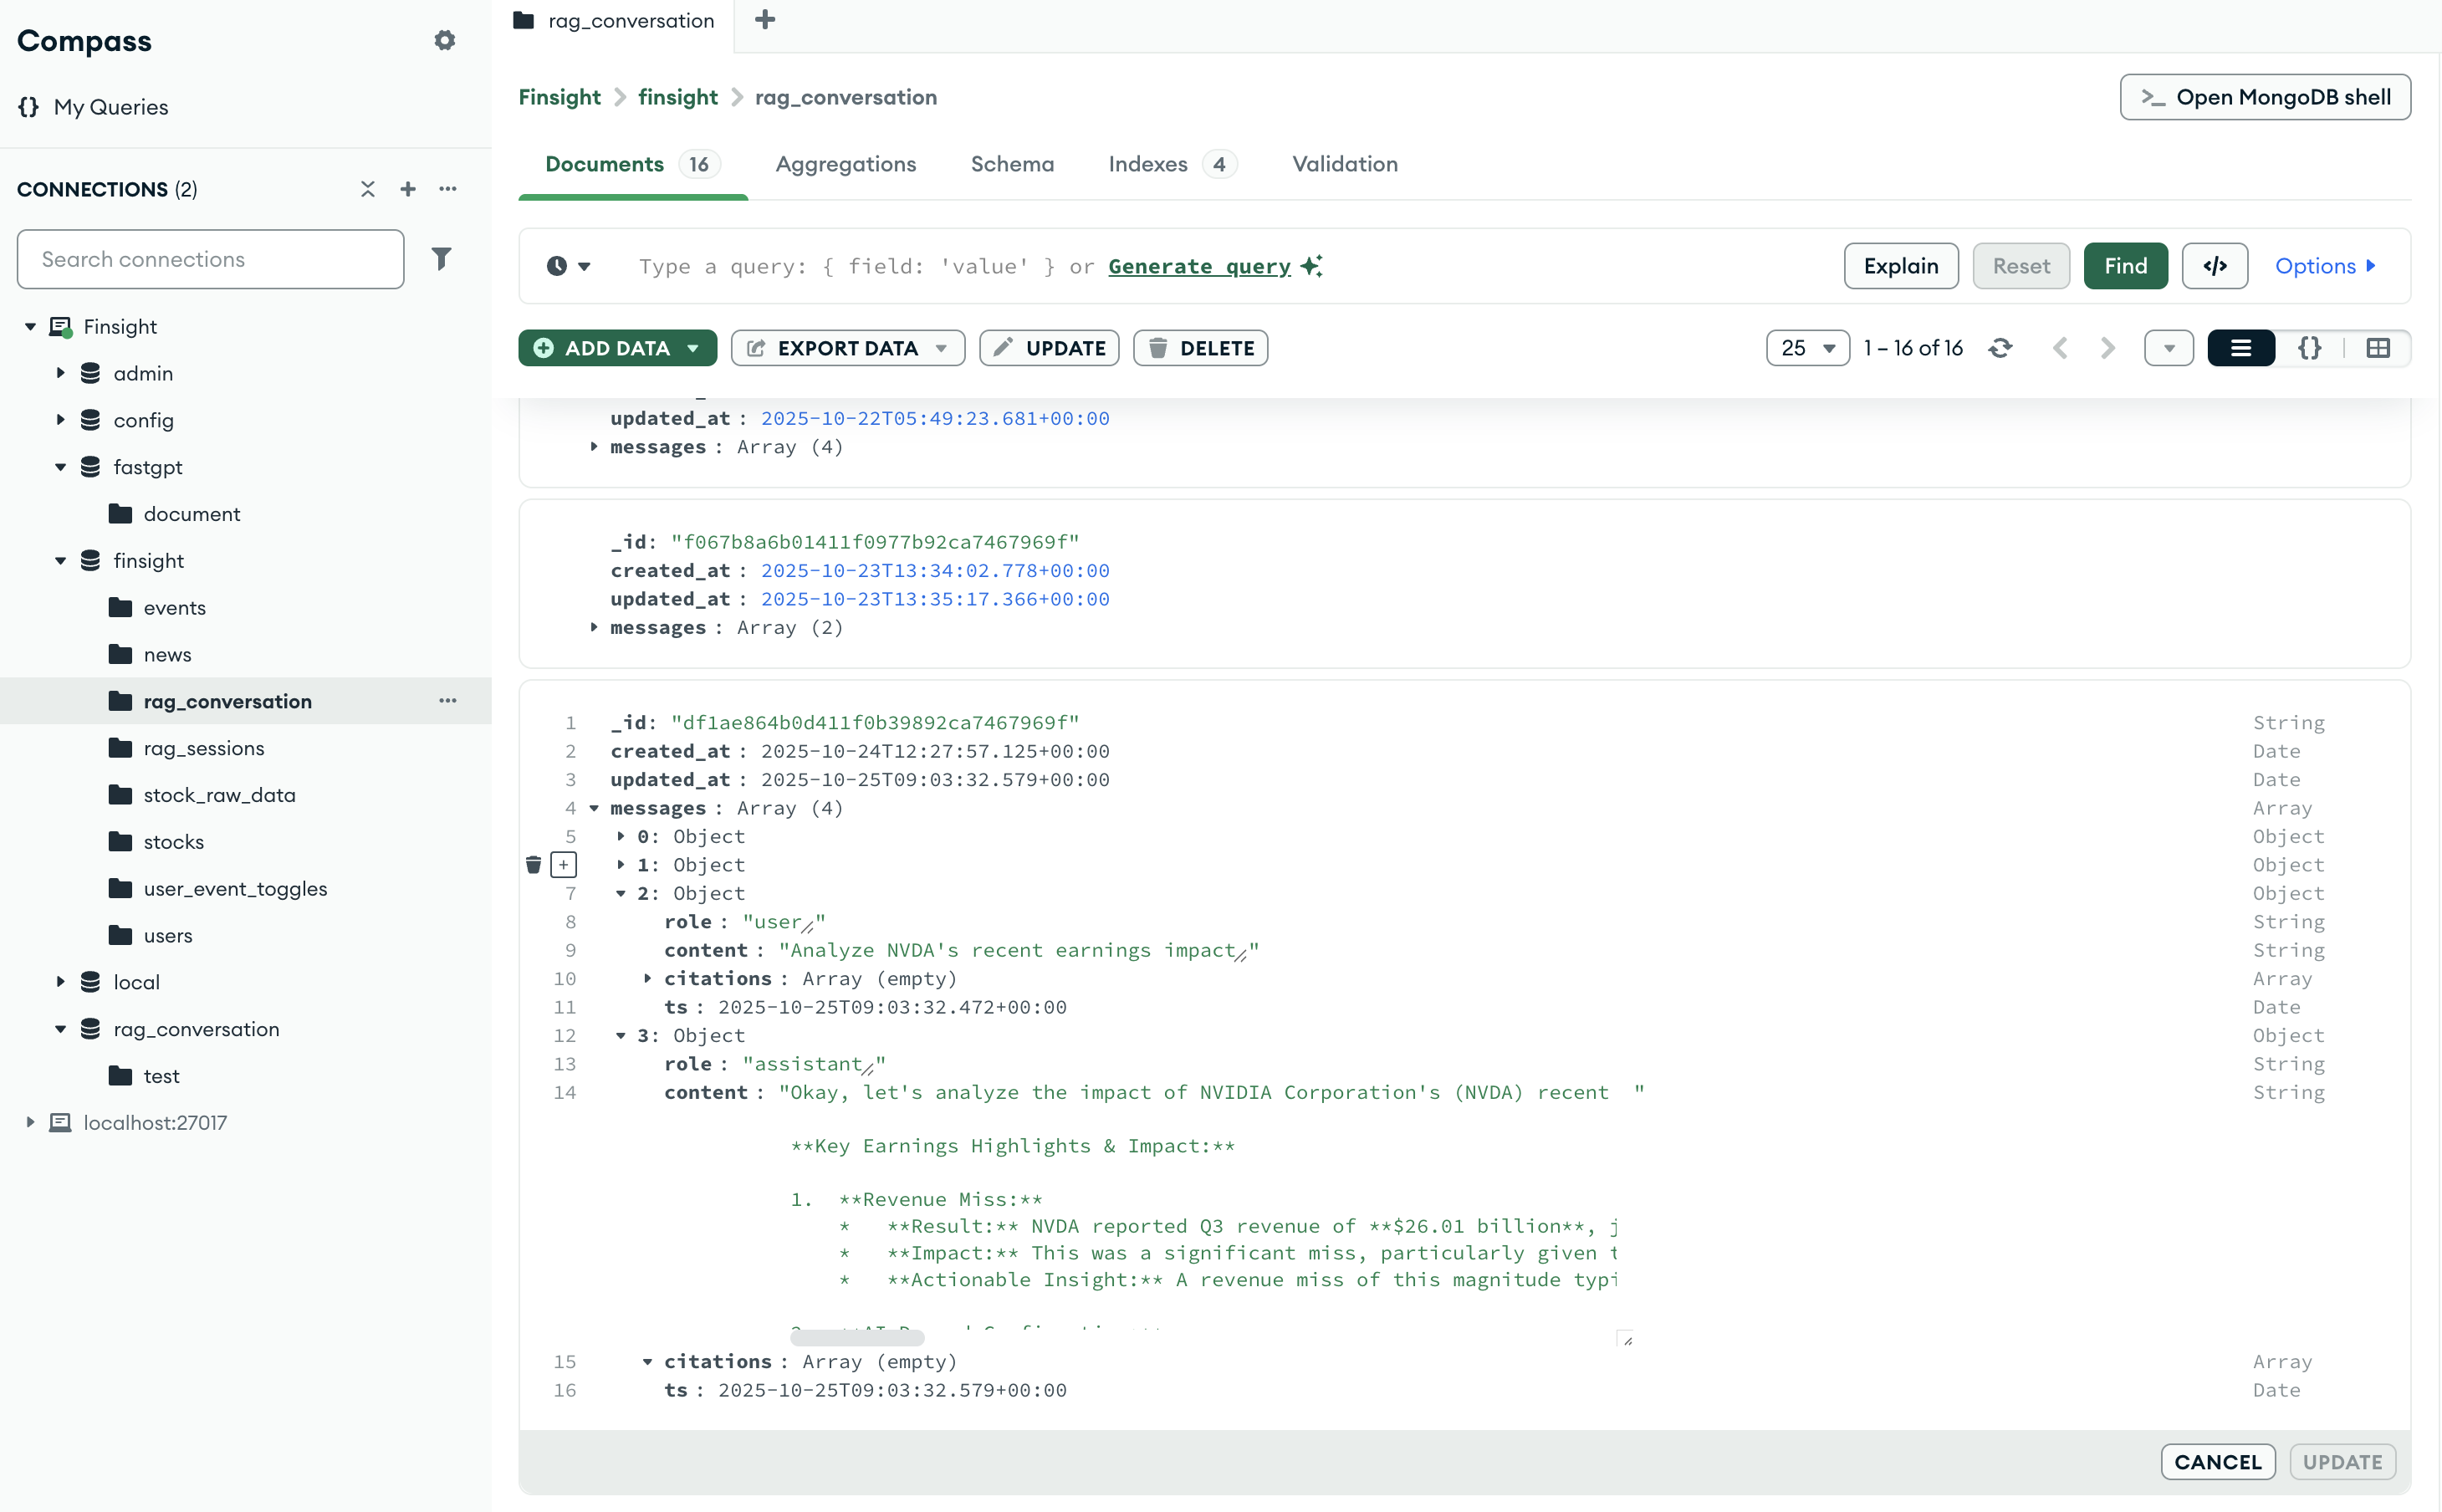
\includegraphics[width=0.75\linewidth]{images/rag_session.png}
    \caption{RAG session and chat history}
\end{center}

\subsection{Prompt Design}
We construct each request with a fixed, evidence-first order to reduce hallucination and keep tone consistent across turns. The system prompt (front-loaded) encodes the grounding policy (summarize from the knowledge base first; disclose fallback reasoning when evidence is thin; keep answers concise and actionable). It is followed by the retrieved knowledge base snippets (de-duplicated and score-truncated), optional recommendation hints (tickers/themes used only as light guidance), and the user query plus minimal session context. This layout ensures KB evidence dominates the model’s attention while recommendations steer specificity without overriding facts; multi-turn continuity is maintained by carrying the session context.

\begin{tcolorbox}
\textbf{System Prompt} \\
\small
\textbf{You are an expert financial research assistant.} Your goal is to provide accurate,
well-reasoned, and context-aware answers using the retrieved knowledge base and your own analytical ability.

\textbf{Instruction:}
1) \textbf{Primary Source:} Prioritize and summarize from the provided knowledge base; cite when relevant. \\
2) \textbf{Fallback Reasoning:} If evidence is insufficient, extend with general financial knowledge and state this explicitly. \\
3) \textbf{Context Awareness:} Respect conversation history and the user’s intent for continuity. \\
4) \textbf{Transparency:} When mainly using general reasoning, begin with a short disclaimer (e.g., “Based on general market understanding…”). \\
5) \textbf{Answer Format:} Be concise and structured; use bullets or short paragraphs; include numbers/dates/ratios and, when appropriate, both \emph{summary} and \emph{implications}.

\medskip
\textbf{Here is the current knowledge base:}

\{knowledge\}

\medskip
When relevant, include market implications or actionable insights (e.g., effects on prices, sectors, or macro indicators).
(If the above is empty or irrelevant, follow the Fallback Reasoning guideline.)
\end{tcolorbox}

Model inputs are concatenated in a fixed order: System Prompt → Knowledge Base Snippet (RAG) → Recommendation Result Prompt (optional, low-weight) → User Question. This design ensures that answers are first summarized based on the retrieved knowledge base, and when insufficient evidence is provided, explicitly triggers the "common market understanding" fallback reasoning, maintaining a consistent tone and context across multiple rounds of dialogue. To reduce hallucinations and redundancy, we deduplicate retrieved snippets, prune them by score, and allocate token budget primarily to knowledge base content. Recommendation prompts retain only symbolic clues to enhance relevance without overriding factual evidence.

\textbf{Conclusion: } The implementation of the AI Analyst subsystem in FinSight successfully integrates retrieval-based factual grounding with generative reasoning to deliver accurate, explainable, and context-aware financial insights. By combining RagFlow’s high-performance retriever and large language model orchestration with FinSight’s modular backend design, the system achieves seamless end-to-end data flow --- from user query submission and document retrieval to structured answer generation and persistent history management. The integration with MongoDB ensures long-term session continuity, while the layered prompt strategy guarantees consistent reasoning behavior and transparency. Overall, the RAG module enhances both the interpretability and reliability of AI-driven financial analysis, enabling users to obtain not only direct answers but also evidence-backed reasoning paths that improve trust and decision confidence.


% \section{Combined Investment Recommendation Module}

% In its initial phase, the module is expected to improve analytic efficiency by reducing the time analysts spend on data collection and cleaning, allowing them to focus more on interpretation. It will produce reports with consistent metrics and transparent assumptions, making peer comparisons easier. Users will be able to respond more quickly to earnings releases, regulatory changes, and macro events, while also gaining better awareness of downside risks through scenario analysis and sensitivity checks. Over time, the system will support benchmarking of its outputs against actual market outcomes, providing a feedback loop on accuracy. For example, for a mid-cap stock, the module should be able to generate valuation estimates reasonably close to market consensus, even within a ±10–20\% range, acknowledging market volatility.


